%% March 2018
%%%%%%%%%%%%%%%%%%%%%%%%%%%%%%%%%%%%%%%%%%%%%%%%%%%%%%%%%%%%%%%%%%%%%%%%%%%%
% AGUJournalTemplate.tex: this template file is for articles formatted with LaTeX
%
% This file includes commands and instructions
% given in the order necessary to produce a final output that will
% satisfy AGU requirements, including customized APA reference formatting.
%
% You may copy this file and give it your
% article name, and enter your text.
%
%
% Step 1: Set the \documentclass
%
% There are two options for article format:
%
% PLEASE USE THE DRAFT OPTION TO SUBMIT YOUR PAPERS.
% The draft option produces double spaced output.
%

%% To submit your paper:
\documentclass[draft]{agujournal2018}

\usepackage{amsmath}
\usepackage{amssymb}

\usepackage{apacite}
\usepackage{url} %this package should fix any errors with URLs in refs.
\usepackage{lineno}
\linenumbers
%%%%%%%
% As of 2018 we recommend use of the TrackChanges package to mark revisions.
% The trackchanges package adds five new LaTeX commands:
%
%  \note[editor]{The note}
%  \annote[editor]{Text to annotate}{The note}
%  \add[editor]{Text to add}
%  \remove[editor]{Text to remove}
%  \change[editor]{Text to remove}{Text to add}
%
% complete documentation is here: http://trackchanges.sourceforge.net/
%%%%%%%

\draftfalse

%% Enter journal name below.
%% Choose from this list of Journals:
%
% JGR: Atmospheres
% JGR: Biogeosciences
% JGR: Earth Surface
% JGR: Oceans
% JGR: Planets
% JGR: Solid Earth
% JGR: Space Physics
% Global Biogeochemical Cycles
% Geophysical Research Letters
% Paleoceanography and Paleoclimatology
% Radio Science
% Reviews of Geophysics
% Tectonics
% Space Weather
% Water Resources Research
% Geochemistry, Geophysics, Geosystems
% Journal of Advances in Modeling Earth Systems (JAMES)
% Earth's Future
% Earth and Space Science
% Geohealth
%
% ie, \journalname{Water Resources Research}

\journalname{Enter journal name here}


\begin{document}

%% ------------------------------------------------------------------------ %%
%  Title
%
% (A title should be specific, informative, and brief. Use
% abbreviations only if they are defined in the abstract. Titles that
% start with general keywords then specific terms are optimized in
% searches)
%
%% ------------------------------------------------------------------------ %%

% Example: \title{This is a test title}

\title{=enter title here=}

%% ------------------------------------------------------------------------ %%
%
%  AUTHORS AND AFFILIATIONS
%
%% ------------------------------------------------------------------------ %%

% Authors are individuals who have significantly contributed to the
% research and preparation of the article. Group authors are allowed, if
% each author in the group is separately identified in an appendix.)

% List authors by first name or initial followed by last name and
% separated by commas. Use \affil{} to number affiliations, and
% \thanks{} for author notes.
% Additional author notes should be indicated with \thanks{} (for
% example, for current addresses).

% Example: \authors{A. B. Author\affil{1}\thanks{Current address, Antartica}, B. C. Author\affil{2,3}, and D. E.
% Author\affil{3,4}\thanks{Also funded by Monsanto.}}

\authors{=list all authors here=}


% \affiliation{1}{First Affiliation}
% \affiliation{2}{Second Affiliation}
% \affiliation{3}{Third Affiliation}
% \affiliation{4}{Fourth Affiliation}

\affiliation{=number=}{=Affiliation Address=}
%(repeat as many times as is necessary)

%% Corresponding Author:
% Corresponding author mailing address and e-mail address:

% (include name and email addresses of the corresponding author.  More
% than one corresponding author is allowed in this LaTeX file and for
% publication; but only one corresponding author is allowed in our
% editorial system.)

% Example: \correspondingauthor{First and Last Name}{email@address.edu}

\correspondingauthor{=name=}{=email address=}

%% Keypoints, final entry on title page.

%  List up to three key points (at least one is required)
%  Key Points summarize the main points and conclusions of the article
%  Each must be 100 characters or less with no special characters or punctuation

% Example:
% \begin{keypoints}
% \item	List up to three key points (at least one is required)
% \item	Key Points summarize the main points and conclusions of the article
% \item	Each must be 100 characters or less with no special characters or punctuation
% \end{keypoints}

\begin{keypoints}
\item enter point 1 here
\item enter point 2 here
\item enter point 3 here
\end{keypoints}

%% ------------------------------------------------------------------------ %%
%
%  ABSTRACT
%
% A good abstract will begin with a short description of the problem
% being addressed, briefly describe the new data or analyses, then
% briefly states the main conclusion(s) and how they are supported and
% uncertainties.
%% ------------------------------------------------------------------------ %%

%% \begin{abstract} starts the second page

\begin{abstract}
enter abstract here

\end{abstract}



%% ------------------------------------------------------------------------ %%
%
%  TEXT
%
%% ------------------------------------------------------------------------ %%

%%% Suggested section heads:
% \section{Introduction}
%
% The main text should start with an introduction. Except for short
% manuscripts (such as comments and replies), the text should be divided
% into sections, each with its own heading.

% Headings should be sentence fragments and do not begin with a
% lowercase letter or number. Examples of good headings are:

% \section{Materials and Methods}
% Here is text on Materials and Methods.
%
% \subsection{A descriptive heading about methods}
% More about Methods.
%
% \section{Data} (Or section title might be a descriptive heading about data)
%
% \section{Results} (Or section title might be a descriptive heading about the
% results)
%
% \section{Conclusions}


\section{Introduction}

Slow slip events are a new feature discovered in the last two decades in many subduction zones thanks to recordings of the displacement of Earth's surface by dense Global Navigation Satellite System (GNSS) networks. As with ordinary earthquakes, slow slip events are caused by slip on a fault, such as the plate boundary between a tectonic plate subducting under another tectonic plate. However, they take a much longer time (several days to several years) to happen relative to ordinary earthquakes, and they have a relatively short recurrence time (months to years), compared to the recurrence time of regular earthquakes (up to several hundreds of years), allowing scientists to observe and study many complete event cycles, which is typically not possible to explore with traditional earthquake catalogs ~\citep{BER_2011}. A slow slip event on the plate boundary is inferred to happen when there is a reversal of the direction of motion at GNSS stations, compared to the secular interseismic motion. Slow slip events have been observed in many subduction zones, such as Cascadia, Nankai (southwest Japan), Alaska, Costa Rica, Mexico, and New Zealand ~\citep{BER_2011,AUD_2016}. \\

In many places, tectonic tremor are also observed in relation to slow slip. Tremor is a long (several seconds to many minutes), low amplitude seismic signal, with emergent onsets, and an absence of clear impulsive phases. Tectonic tremor have been explained as a swarm of small, low-frequency earthquakes (LFEs) ~\citep{SHE_2007_nature}, that is small magnitude earthquakes (M $\sim$ 1), for which frequency content (1-10 Hz) is lower than for ordinary earthquakes (up to 20 Hz). In subduction zones such as Nankai and Cascadia, tectonic tremor observations are spatially and temporally correlated with slow slip observations~\citep{OBA_2002,ROG_2003}. Due to this correlation, these paired phenomena have been called Episodic Tremor and Slip (ETS). However, this is not always the case. For instance, in northern New Zealand, tremor are more challenging to detect, and seem to be located downdip of the slow slip on the plate boundary. \\

In Cascadia and Guerrero, Mexico, tremor has been used as a proxy to observe slow slip events that are not directly detectable in the GNSS data. For instance, ~\citet{AGU_2009} computed the GPS-estimated moment release for 23 ETS events in Cascadia between 1997 and 2008. Simultaneously, they computed the cumulative number of hours of tectonic tremor recorded for each event. They observed a linear relationship between moment release and number of hours of tremor for ETS events of moment magnitude 6.3 to 6.8. For all these events, at least 50 hours of tectonic tremor where observed simultaneously with the GPS deformation. However, many smaller bursts of tremor of duration 1 to 50 hours were also observed in between the big ETS events. Based on the relationship between slow slip moment and number of hours of tremor, ~\citet{AGU_2009} suggested that smaller slow slip events of magnitude 5-6 may occur simultaneously with the tremor bursts without being detectable in the GPS data. \\

~\citet{FRA_2016} transformed the GPS time series into daily increments of surface motion by computing the first order differentiation of the time series. He then discarded the daily increments observed during known big slow slip events, and focused on the inter-events period. He divided the daily increments into two groups: the first group contains days when slow seismicity (tectonic tremor and LFEs) is detected, the second group contains days when the numbers of LFEs (for Guerrero) or tremor (for Cascadia) is lower than a threshold. He then stacked separately the two groups of daily increments and observed a cumulative displacement in the northern direction (for Guerrero) and the eastern direction (for Cascadia) corresponding to the loading period when few tremor or LFEs are observed and the surface deformation corresponds to the secular plate motion. He also observed a cumulative displacement in the southern direction (for Guerrero) and the western direction (for Cascadia) corresponding to the release period when tremor and LFEs are observed. This reverse displacement corresponds to smaller slow slip events not directly observable in the GPS data.  \\

However, in other subduction zones such as New Zealand, there is no clear relationship between tremor and slow slip occurrence and these methods cannot be applied. We thus need other methods to be able to better detect and quantify slow slip. \\

Wavelets methods such as the Discrete Wavelet Transform (DWT) are mathematical tools for analyzing time series simultaneously in the time and the frequency domain by observing how weighted averages of a time series vary from one averaging period to the next. Wavelet methods have been widely used for geophysical applications ~\citep{KUM_1997}. However, few studies have used wavelet methods to analyze recordings of slow slip, and their scope was limited to the detection of the bigger (magnitude 6-7) short-term (a few weeks) events. \\

~\citet{ALB_2019} used hourly water level records from four tide gauges in the Juan de Fuca Straight and the Puget Sound to determine vertical displacements, uplift rates between ETS events, and net uplift rates between 1996 and 2011. The noise in the tide gauges data is associated with tides, and ocean and atmospheric noise on multiple timescales (a few days for storms to decades for oscillations between ocean basins), and is assumed to be coherent between each of the four tidal gauges studied. On the contrary, the uplift due to ETS events should be different at each tidal gauge. They first removed the tides using NOAA hourly harmonic tidal predictions. They then removed the residual noise using a method based on the DWT. More precisely, the authors applied a DWT to each of the four sites studied, and to the average of the four sites. Then, for each level of the DWT decomposition, they carried out a linear regression between the detail for one site and the detail for the average of the four sites. This process gives a coefficient for each level and for each site. They then constructed a noise signal for each site by multiplying the coefficient from the linear regression by the detail of the average over the four sites, and summing for all levels. The noise signal thus obtained was then removed from the time series. They then stacked multiple events to obtain an average event uplift rate, aligning the 12 ETS events using exact timing from GPS data. A difference in uplift between the two tidal gauges at Port Angeles and Port Townsend was then clearly seen in the stacked time series. Finally, the authors removed the long-term uplift rate and the long-term sea level rise to obtain an average inter-event uplift rate. They found that the inter-event deformation at a site is equal and opposite to the deformation during an ETS event, suggesting that ETS events are, on average, releasing the strain accumulated between ETS events. \\

~\citet{SZE_2008} determined the timing and the amplitude of 34 slow slip events throughout the Cascadia subduction zone between 1997 and 2005. They stabilized the GPS time series using a reference set of stations from stable North America. They then modelled the GPS time series by the sum of a linear trend, annual and biannual sinusoids representing seasonal effects, and Heaviside step functions corresponding to earthquakes and hardware upgrades. The linear system was then solved using a weighted QR decomposition. Finally, they applied a Gaussian wavelet transform to the residual time series to get the exact timing of the slow slip at each GPS station. The succeeding wavelet basis functions are increasingly sensitive to temporal localization of a given signal, and the onset of faulting appears on the wavelet spectrum as an amplitude spike present over all frequencies. The offset for each slow slip event was then used to invert for the slow slip at depth by assuming a thrust fault slip at each subfault of the plate boundary. An equivalent moment magnitude was thus obtained. \\

Finally, instead of using wavelets in the time domain, ~\citet{OHT_2010} used 2D wavelet functions in the spatial domain to detect slow slip events. They designed the Network Stain Filter (NSF) to detect transient deformation signals from large-scale geodetic arrays. Contrary to their previous work on the Network Inversion Filter (NIF), there is no need to specify potential sources of deformation. They modeled the position of the GPS station by the sum of the secular velocity, a spatially coherent field, site-specific noise, reference frame errors, and observation errors. The spatial displacement field is modeled by the sum of basis wavelets (the Deslauriers-Dubuc wavelet of degree 3) with time-varying weights. The transient is considered to be nearly steady-sate, so that it has spatial weights for the displacement and the velocity, but the acceleration is modeled by a random walk with a time-varying variance. All the time varying coefficients are estimated using Kalman filtering, and the optimization problem is regularized with the spatial sum of the transient strain rate field. Their method has been successfully used to detect a transient event in the Boso peninsula, Japan, and a slow slip event in the Alaska subduction zone ~\citep{WEI_2012}. \\

In this study, we use wavelet methods to analyze GPS and seismic recordings of slow slip events in Cascadia. Our objective is to verify that there is a good correlation between slow slip events detected with only GNSS data, and slow slip events detected with only seismic data. We thus want to demonstrate that the wavelet-based detection method can be applied to detect slow slip events that may be currently undetected with standard methods. \\

\section{Data}

We focused our study on northwest Washington State. For the GNSS data, we used the GPS time series provided by the Pacific Northwest Geodetic Array, Central Washington University. These are network solutions in ITRF2008 with phase ambiguities resolved. Solutions are computed with JPL/NASA orbits and satellite clocks. North, East, and Vertical directions are available. However, as the direction of the secular plate motion is close to the East direction, we only used the East direction of the GPS time series for the data analysis, as it has the best signal-to-noise ratio. The wavelet method works best with data with zero mean, and no sharp discontinuities, so we use the cleaned dataset, that is GPS times eries with linear trends, steps due to earthquakes or hardware upgrades, and annual and semi-annual sinusoids signals simultaneously estimated and removed following ~\citet{SZE_2004}. For the seismic data, we used the tremor catalog from the Pacific Northwest Seismic Network (PNSN) ~\citep{WEC_2010}. Tremor were detected and located using waveform envelope correlation and clustering and a centroid location is available for every given five-minute time window when tremor was detected. As the catalog starts in August 2009, we only looked at GPS data recorded in 2009 or later. \\

\section{Method} 

\subsection{The Maximal Overlap Discrete Wavelet Transform}

The Discrete Wavelet Transform (DWT) is an orthonormal transform that transforms a time series $X_t \left( t = 0, \cdots , N - 1 \right)$ into a vector of wavelet coefficients $W_i \left( i = 0 , \cdots , N - 1 \right)$. If we denote $J$ the level of the wavelet decomposition, and we have $N = n * 2^J$, where $n$ is some integer higher or equal to 1, the vector of wavelet coefficients can be decomposed into $J$ wavelet vectors $W_j$ of lengths $\frac{N}{2}$, $\frac{N}{4}$, ... , $\frac{N}{2^J}$, and one scaling vector $V_J$ of length $\frac{N}{2^J}$. Each wavelet vector $W_j$ is associated with changes on scale $\tau_j = dt 2^{j - 1}$, where $dt$ is the time step of the time series, and corresponds to the filtering of the original time series with a filter with nominal frequency interval $\lbrack \frac{1}{dt 2^{j + 1}} ; \frac{1}{dt 2^j} \rbrack$. The scaling vector $V_J$ is associated with averages in scale $\lambda_J = dt 2^J$, and corresponds to the filtering of the original time series with a filter with nominal frequency interval $\lbrack 0 ; \frac{1}{dt 2^{j + 1}} \rbrack$. We can also define for $j = 1 , \cdots , J$ the $j$th wavelet detail $D_j$, which is a vector of length $N$, and is associated to scale $\tau_j = dt 2^{j - 1}$. Similarly, we can define for $j = 1 , \cdots , J$ the $j$th wavelet smooth $S_j$, which is a vector of length $N$, and is associated to scales $\tau_{j + 1} = dt 2^{j + 1}$ and higher. Together, the details and the smooths define the multiresolution analysis (MRA) of $X$:

\begin{linenomath*}
\begin{equation}
X = \sum_{j = 1}^{J} D_j + S_J
\end{equation}
\end{linenomath*}

The DWT present several disadvantages. First, the length of the time series must be a multiple of $2^J$ where $J$ is the level of the DWT decomposition. Second, the time step of the wavelet vector $W_j$ is $dt 2^j$, which may not correspond to the time when some interesting phenomenon is visible on the original time series. Third, when we circularly shift the time series, the corresponding wavelet coefficients, details and smooths are not a circularly shifted version of the wavelet coefficients, details and smooths of the original time series. Thus, the values of the wavelet coefficients, details and smooths are strongly dependent on the time when we start experimentally gathering the data. Finally, when we filter the time series to obtain the details and smooths, we introduce a phase shift, which makes difficult to line up meaningfully the features of the MRA with the original time series. \\

This is why we use instead the Maximal Overlap Discrete Wavelet Transform (MODWT). The MODWT transforms the time series $X_t \left( t = 0, ... , N - 1 \right)$ into J wavelet vectors $\widetilde{W}_j \left( j = 1 ,  \cdots , J \right)$ of length $N$ and a scaling vector $\widetilde{V}_J$ of length $N$. As is the case for the DWT, each wavelet vector $\widetilde{W}_j$ is associated with changes on scale $\tau_j = dt 2^{j - 1}$, and corresponds to the filtering of the original time series with a filter with nominal frequency interval $\lbrack \frac{1}{dt 2^{j + 1}} ; \frac{1}{dt 2^j} \rbrack$. The scaling vector $\widetilde{V}_J$ is associated with averages in scale $\lambda_J = dt 2^J$, and corresponds to the filtering of the original time series with a filter with nominal frequency interval $\lbrack 0 ; \frac{1}{dt 2^{j + 1}} \rbrack$. As is the case for the DWT, we can write the MRA:

\begin{linenomath*}
\begin{equation}
X = \sum_{j = 1}^{J} \widetilde{D}_j + \widetilde{S}_J
\end{equation}
\end{linenomath*}

The MODWT of a time series can be defined for any length $N$. The time step of the wavelet vectors $\widetilde{W}_j$ and the scaling vector $\widetilde{V}_J$ is equal to the time step of the original time series. When we circularly shift the time series, the corresponding wavelet vectors, scaling vector, details and smooths are shifted by the same amount. The details and smooths are associated with a zero phase filter, making it easy to line up meaningfully the features of the MRA with the original time series. The wavelet methods for time series analysis are explained in a more detailed way in ~\citet{PER_2000}). \\

\subsection{Application to synthetic data}

To illustrate the wavelet transform method, we first apply the MODWT to synthetics data. As slow slip events occur in Cascadia on a regular basis, every twelve to eighteen months, we create a synthetic signal of period $T = 500$ days. To reproduce the ground displacement observed on the longitudinal component of GPS stations in Cascadia, we divide each period into two parts: In the first part of duration $T - N$, the displacement is linearly increasing and corresponds to the secular plate motion in the eastern direction; in the second part of duration $N$, the displacement is linearly decreasing and corresponds to a slow slip event on a reverse fault at depth triggering a ground displacement in the western direction. To see the effect of the magnitude of the slow slip event, we use different values for $N = 2, 5, 10, 20$ days. Figure 1 shows the synthetics, the details of the wavelet decomposition for levels 1 to 8, and the smooth for the four durations of a slow slip event. \\

\begin{figure}
\noindent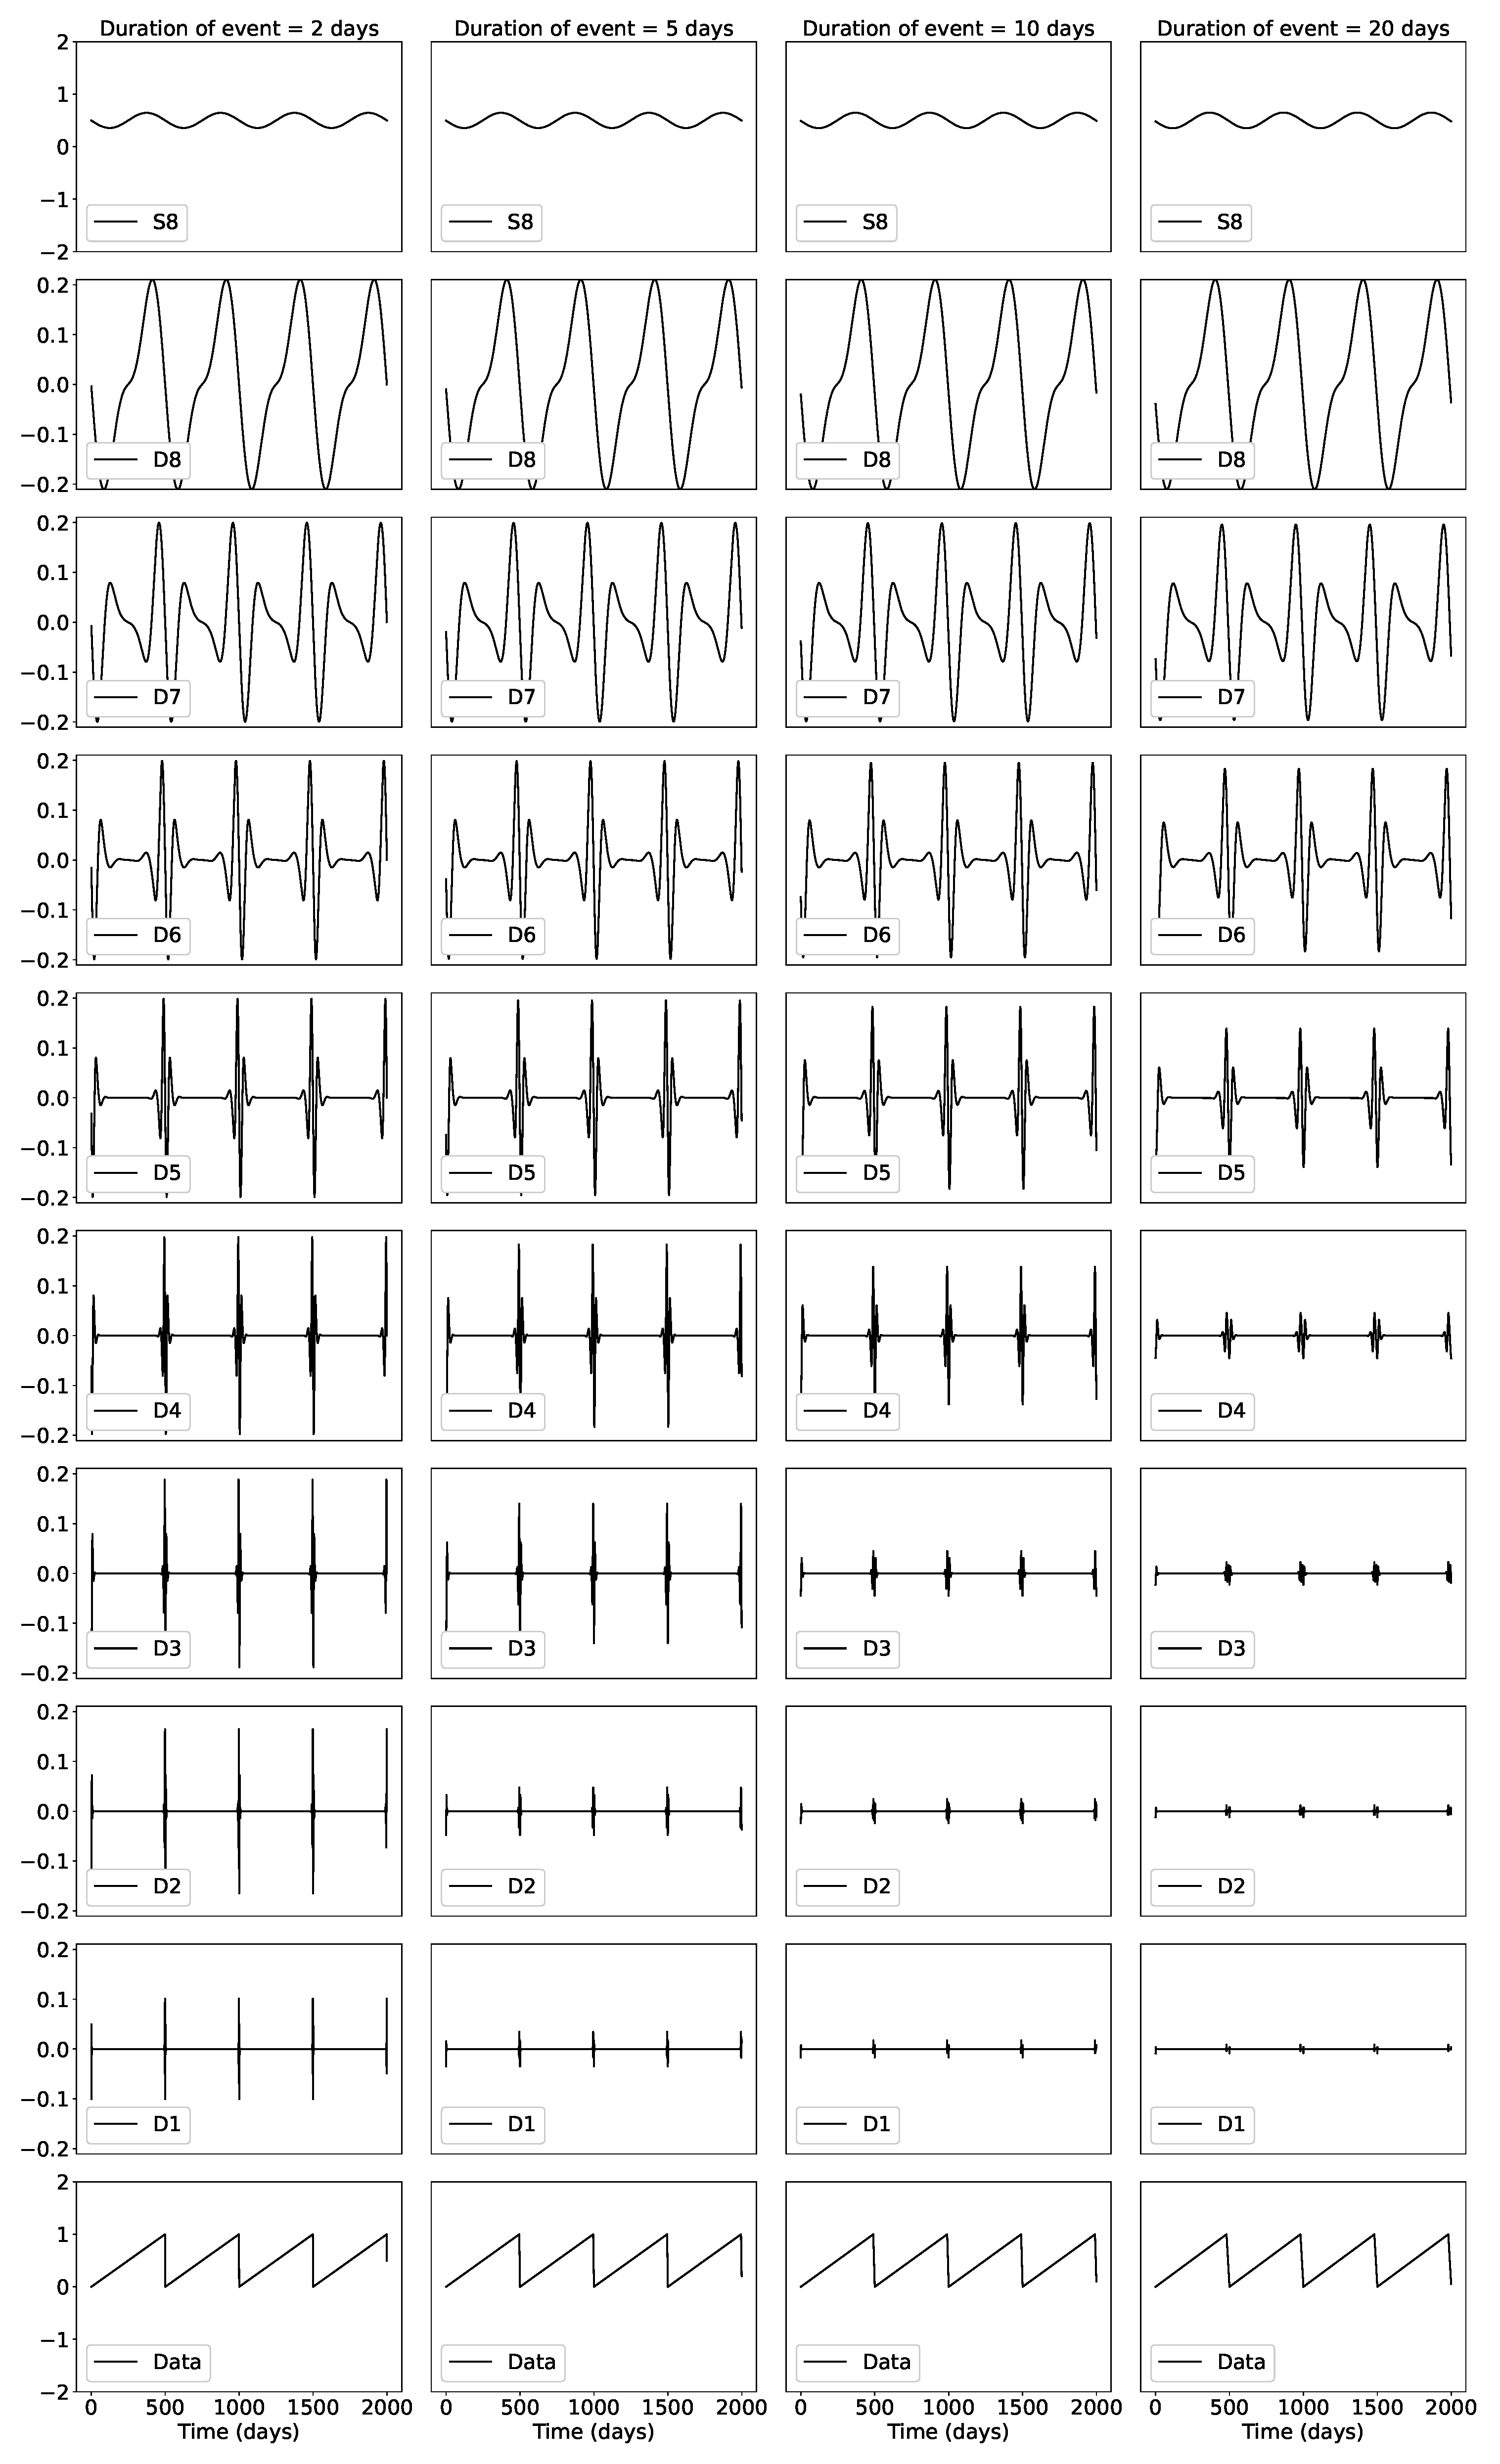
\includegraphics[width=\textwidth, trim={0cm 0cm 0cm 0cm},clip]{figures/500_DS.eps}
\caption{Details and smooth of the wavelet decomposition of a synthetics signal with period 500 days and duration of the slow slip event equal to 2 days (left), 5 days, 10 days, and 20 days (right).}
\label{pngfiguresample}
\end{figure}

The ramp-like signal is transformed through the wavelet filtering into a waveform with first a positive peak and then a negative peak. The width of the waveform increases with the scale level. For the 8th level of the wavelet decomposition, the width of the waveform is nearly as large as the time between two events. We do not show details at larger scales as the corresponding waveforms would start to merge two contiguous events together, and make the wavelet decomposition less interpretable. For an event of duration 2 days, the wavelet details at levels higher than 2 have a larger amplitude than the wavelet detail at level 1. For an event of duration 5 days, the wavelet details at levels higher than 3 have a larger amplitude than the wavelet details at lower scales. For an event of duration 10 days, the wavelet details at levels higher than 5 have a larger amplitude than the wavelet details at lower scales. For an event of duration 20 days, the wavelet details at levels higher than 6 have a larger amplitude than the wavelet details at lower scales. Thus, the scale levels at which an event is being seen in the wavelet details give us an indication about the duration (and the magnitude) of the slow slip event. We expect the big slow slip events of magnitude 6-7 that lasts about 10 days to start being visible at the level 5 of the wavelet decomposition, but to not be noticeable at lower time scales. \\

\subsection{MODWT of GPS and tremor data}

The DWT and MODWT methods must be used on a continuous time series, without gaps in the recordings. To deal with the gaps in the GNSS recordings, we simply replace the missing values by Gaussian noise with mean zero and standard deviation equal to the standard deviation of the whole time series. We verify how the wavelet details may be affected by looking at a GPS time series without missing values and comparing the wavelet details with and without removing some data points. Station PGC5 has recorded during 1390 days between 2009 and 2013, without any missing values. We first computed the wavelet details without missing values. Then, we removed ten neighboring missing values, replaced them by Gaussian noise, and computed the wavelet details with the replaced values. Figure 2 shows a comparison of the two wavelet details for two different locations of the missing values. We can see that there are visible differences in the time series itself, and in the details at the smallest levels of the wavelet decomposition. However, the differences between the wavelet details with and without missing values get smaller and smaller with increasing levels the details, and are barely visible for the levels we are mostly interested in (levels 6 to 8). We thus conclude that we can easily replace the missing values in the GNSS time series without introducing false detections of slow slip events. \\

\begin{figure}
\noindent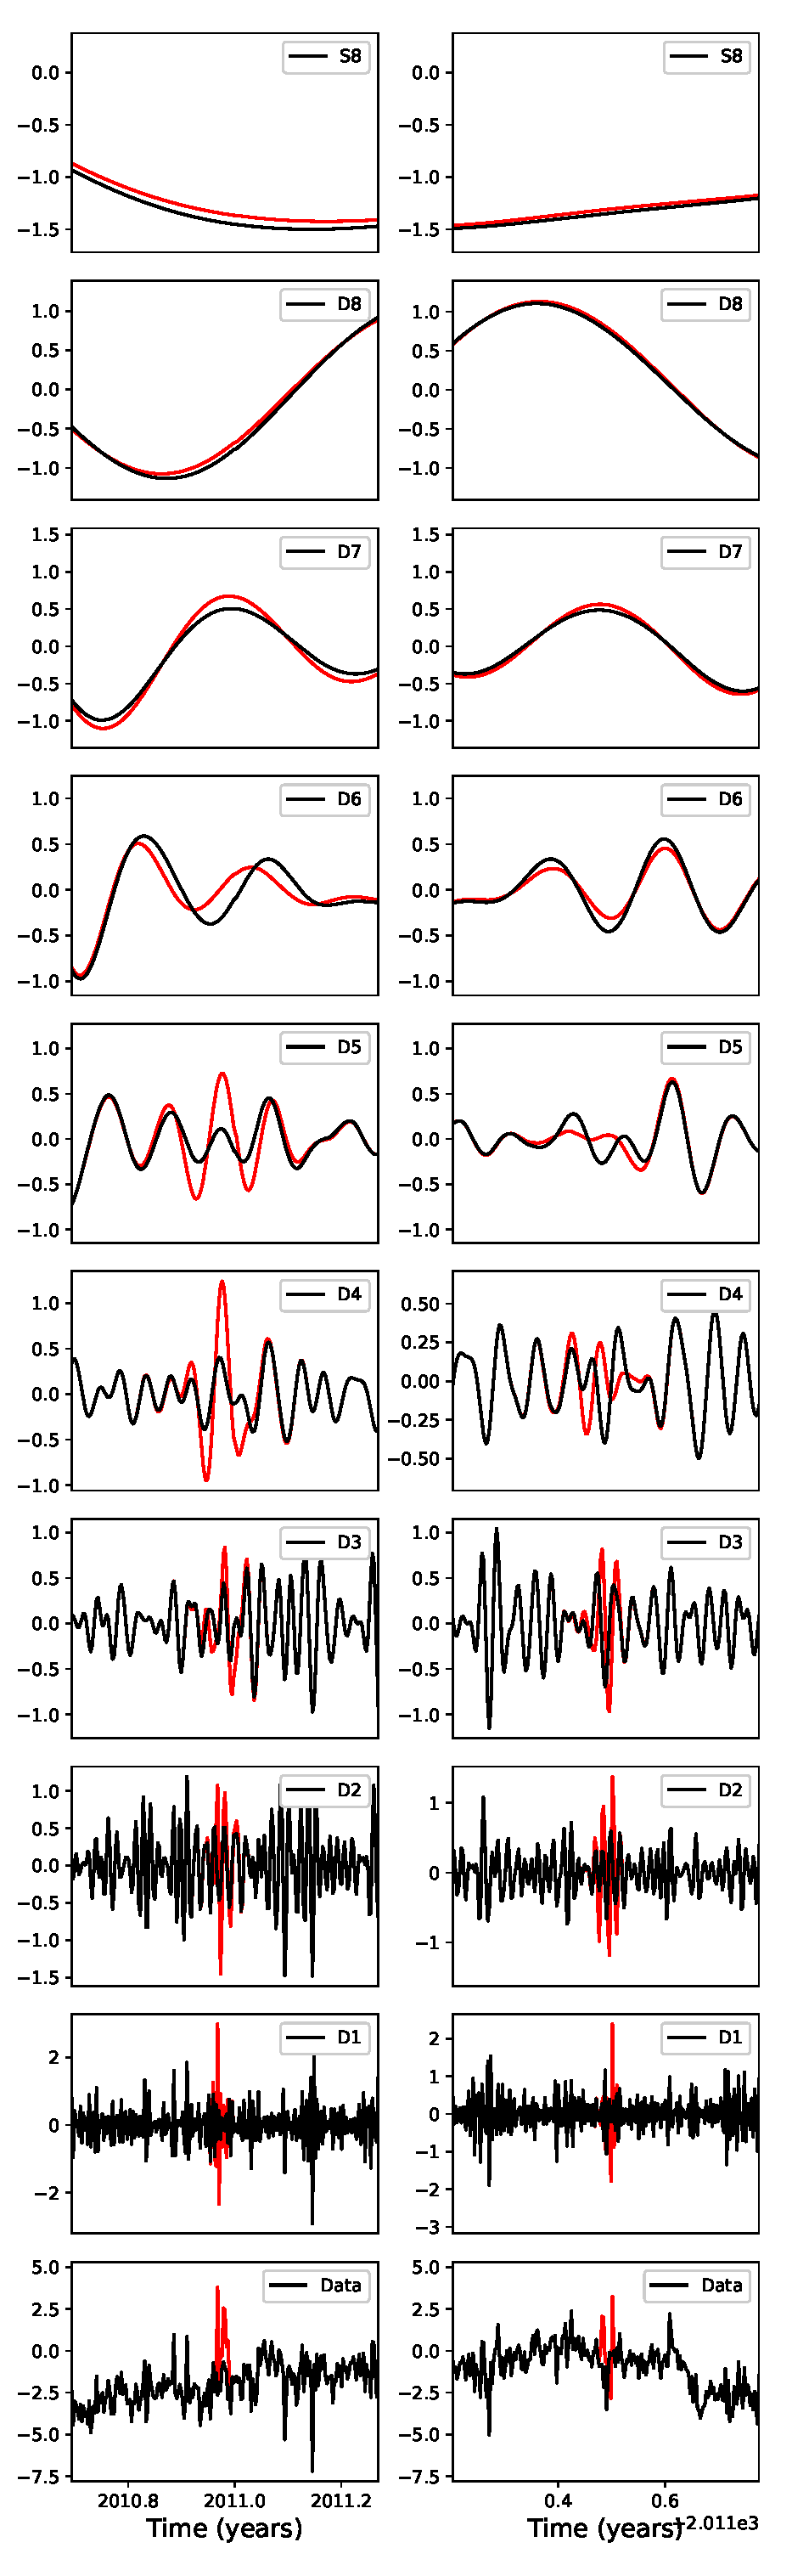
\includegraphics[width=5cm, trim={0cm 0cm 0cm 0cm},clip]{figures/DS_10.eps}
\caption{Bottom: Data from GPS station PGC5 without missing values (black) and with missing values replaced by Gaussian noise (red) for two locations of the missing values (left and right). Bottom to top: Corresponding eight details and smooths of the wavelet composition for the original data (black) and for the missing values replaced by Gaussian noise (red).}
\label{pngfiguresample}
\end{figure}

We then applied the wavelet filtering to real GPS data. Figure 3 shows the longitudinal displacement for GPS station PGC5, located in southern Vancouver Island, the details of the wavelet decomposition for levels 1 to 8, and the smooth. In the data, we can see a sharp drop in displacement whenever there is a slow slip event. For levels 5 to 8, we can see in the details a positive peak followed by a negative peak whenever there is a drop in displacement in the data. We thus verify that the wavelet method can detect slow slip events. \\

\begin{figure}
\noindent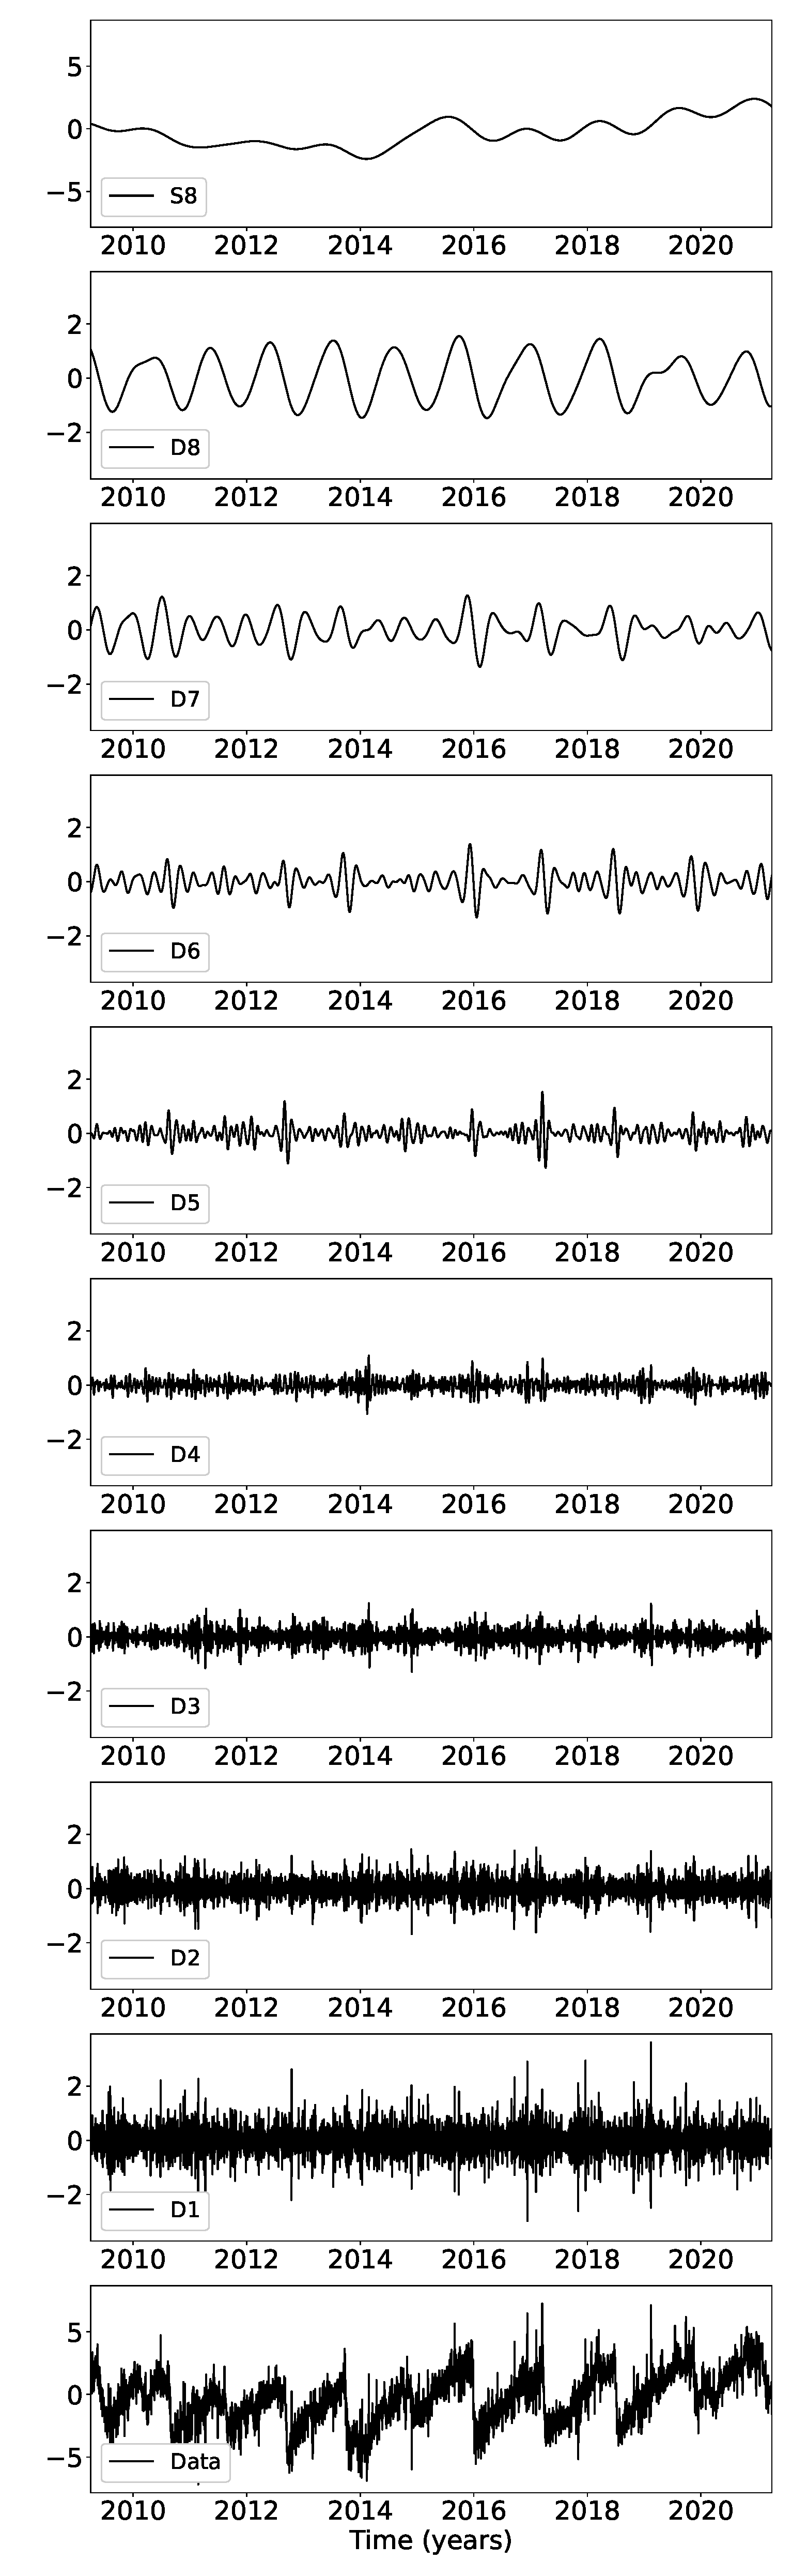
\includegraphics[width=5cm, trim={0cm 0cm 0cm 0cm},clip]{figures/cleaned_PGC5_lon.eps}
\caption{Details and smooth of the wavelet decomposition of the longitudinal displacement recorded at GPS station PGC5.}
\label{pngfiguresample}
\end{figure}

To increase the signal-to-noise ratio and be able to better detect slow slip events, we stack the signal over several GPS stations. We choose to focus on GPS stations located close enough to the tremor zone to get a sufficiently high amplitude of the slow slip signal. We choose 16 points located on the 40 km depth contour of the plate boundary (model from ~\citet{PRE_2003}) with spacing equal 0.1 degree in latitude (red triangles on Figure 4). Then we took all the GPS stations located in a 50 km radius for a given point, compute the wavelet details for the longitudinal displacement of each station, and stack each detail over the GPS stations. We thus have a stacked detail for each level 1 to 8 of the wavelet decomposition. \\

\begin{figure}
\noindent\includegraphics[width=\textwidth, trim={0cm 0cm 0cm 0cm},clip]{figures/map_GPS_stations.eps}
\caption{GPS stations used in this study (black triangles). The black line represents the 40 km depth contour of the plate boundary model by ~\citet{PRE_2003}. The red triangles are the locations where we stack the GPS data. The small grey dots are all the tremor locations from the PNSN catalog.}
\label{pngfiguresample}
\end{figure}

To compare slow slip events detected with GPS data and slow slip events detected with seismic data, we took all the tremor epicenters located within a 50 km radius centered on one of the 16 locations marked by red triangles on Figure 3. Then we computed the cumulative number of tremor within this circle. Finally, we removed a linear trend from the cumulative tremor count, and applied the wavelet transform. Figure 5 shows an example of the wavelet decomposition for the third northernmost location on Figure 4 (which is closest to GPS station PGC5). Contrary to what happens for the GPS data, we see a sharp increase in the data whenever there is a tremor episode, which translates into a negative peak followed by a positive peak in the wavelet details.

\begin{figure}
\noindent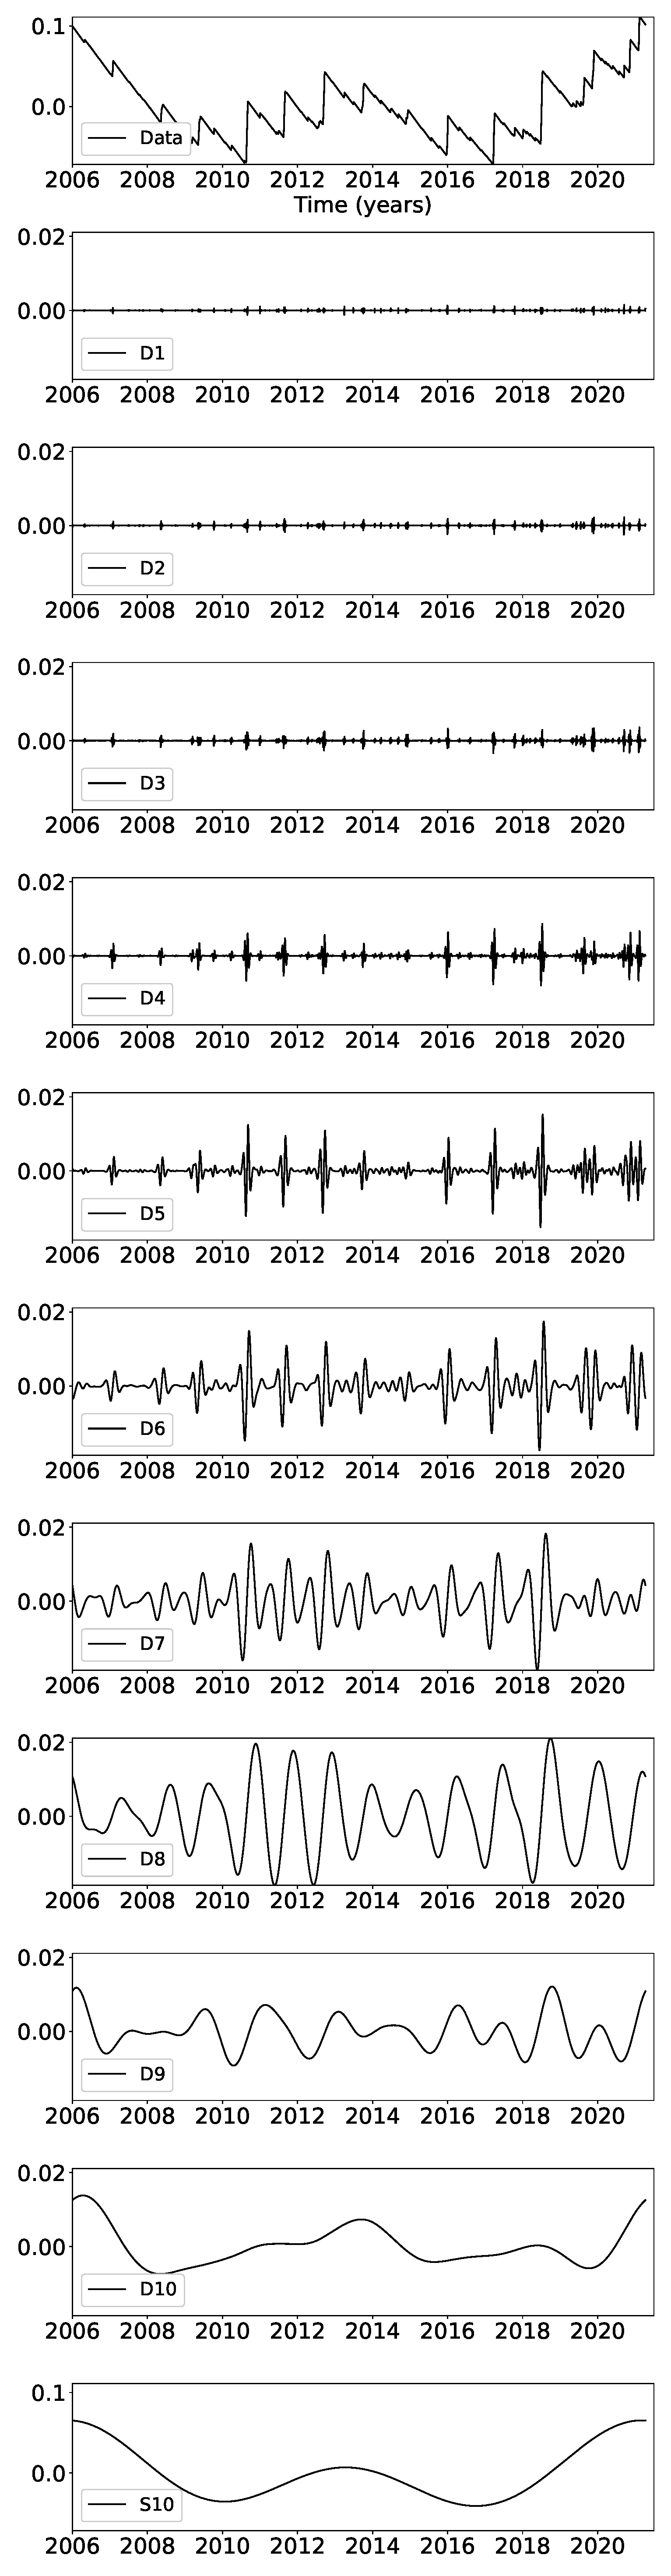
\includegraphics[width=5cm, trim={0cm 0cm 0cm 0cm},clip]{figures/tremor_13.eps}
\caption{Details and smooth of the wavelet decomposition of the detrended cumulative tremor count around the third northernmost location on Figure 3.}
\label{pngfiguresample}
\end{figure}

\section{Results}

We stacked the 8th level detail of the wavelet decomposition of the displacement over all the GPS stations located in a 50 km radius of a given point, for the 16 locations indicated in Figure 3. The result is shown in the top panel of Figure 6, where each line represents one of the locations. To better highlight the peaks in the wavelet details, we highlighted in red the time intervals where the amplitude of the stacked detail is higher than a threshold, and in blue the  time intervals where the amplitude of the stacked detail is lower than minus the threshold. To compare the GPS signal with the tremor signal, we plotted the 8th level detail of the wavelet decomposition of the tremor count on the bottom panel of Figure 6. We used the opposite of the cumulative tremor count for the wavelet decomposition in order to be able to match positive peaks with positive peaks and negative peaks with negative peaks. Although the latitudinal extension of the events is not always the same for the GPS data and for the tremor data, we identify the same 10 events in both 8th wavelet decompositions for the 8th level: Summer 2010, Summer 2011, Summer 2012, Fall 2013, Summer-Fall 2014, Winter 2015-2016, Winter 2017, Spring 2018, Spring-Fall 2019, and Fall 2020 - Winter 2021. We can also see the end of an 11th event in Summer 2009. \\

\begin{figure}
\noindent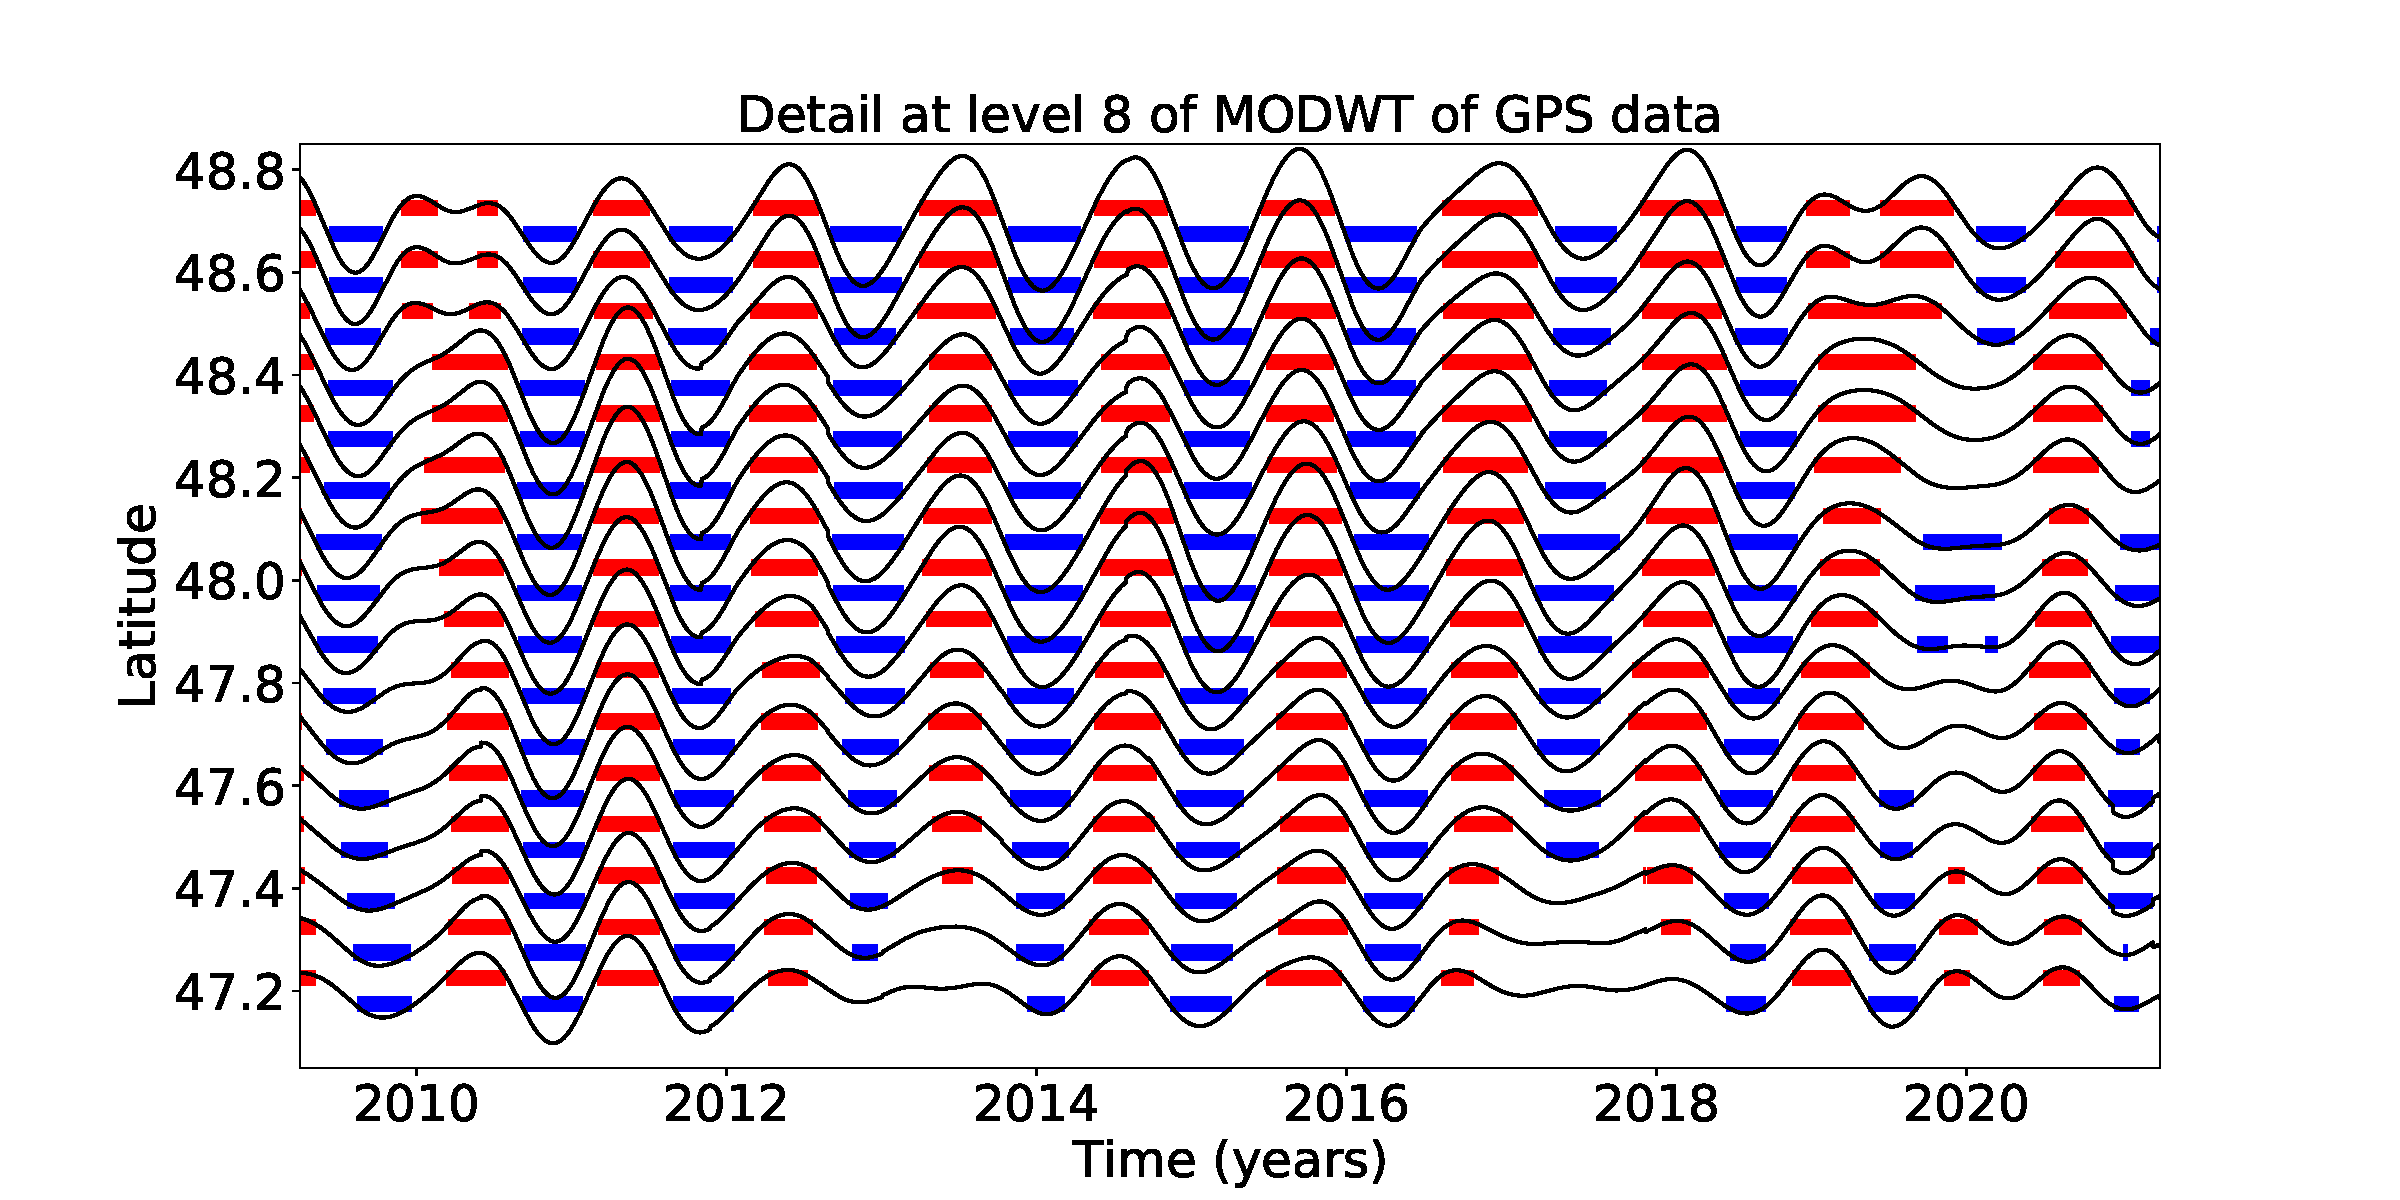
\includegraphics[width=\textwidth, trim={0cm 0cm 0cm 0cm},clip]{figures/GPS_detail_8.pdf}

\noindent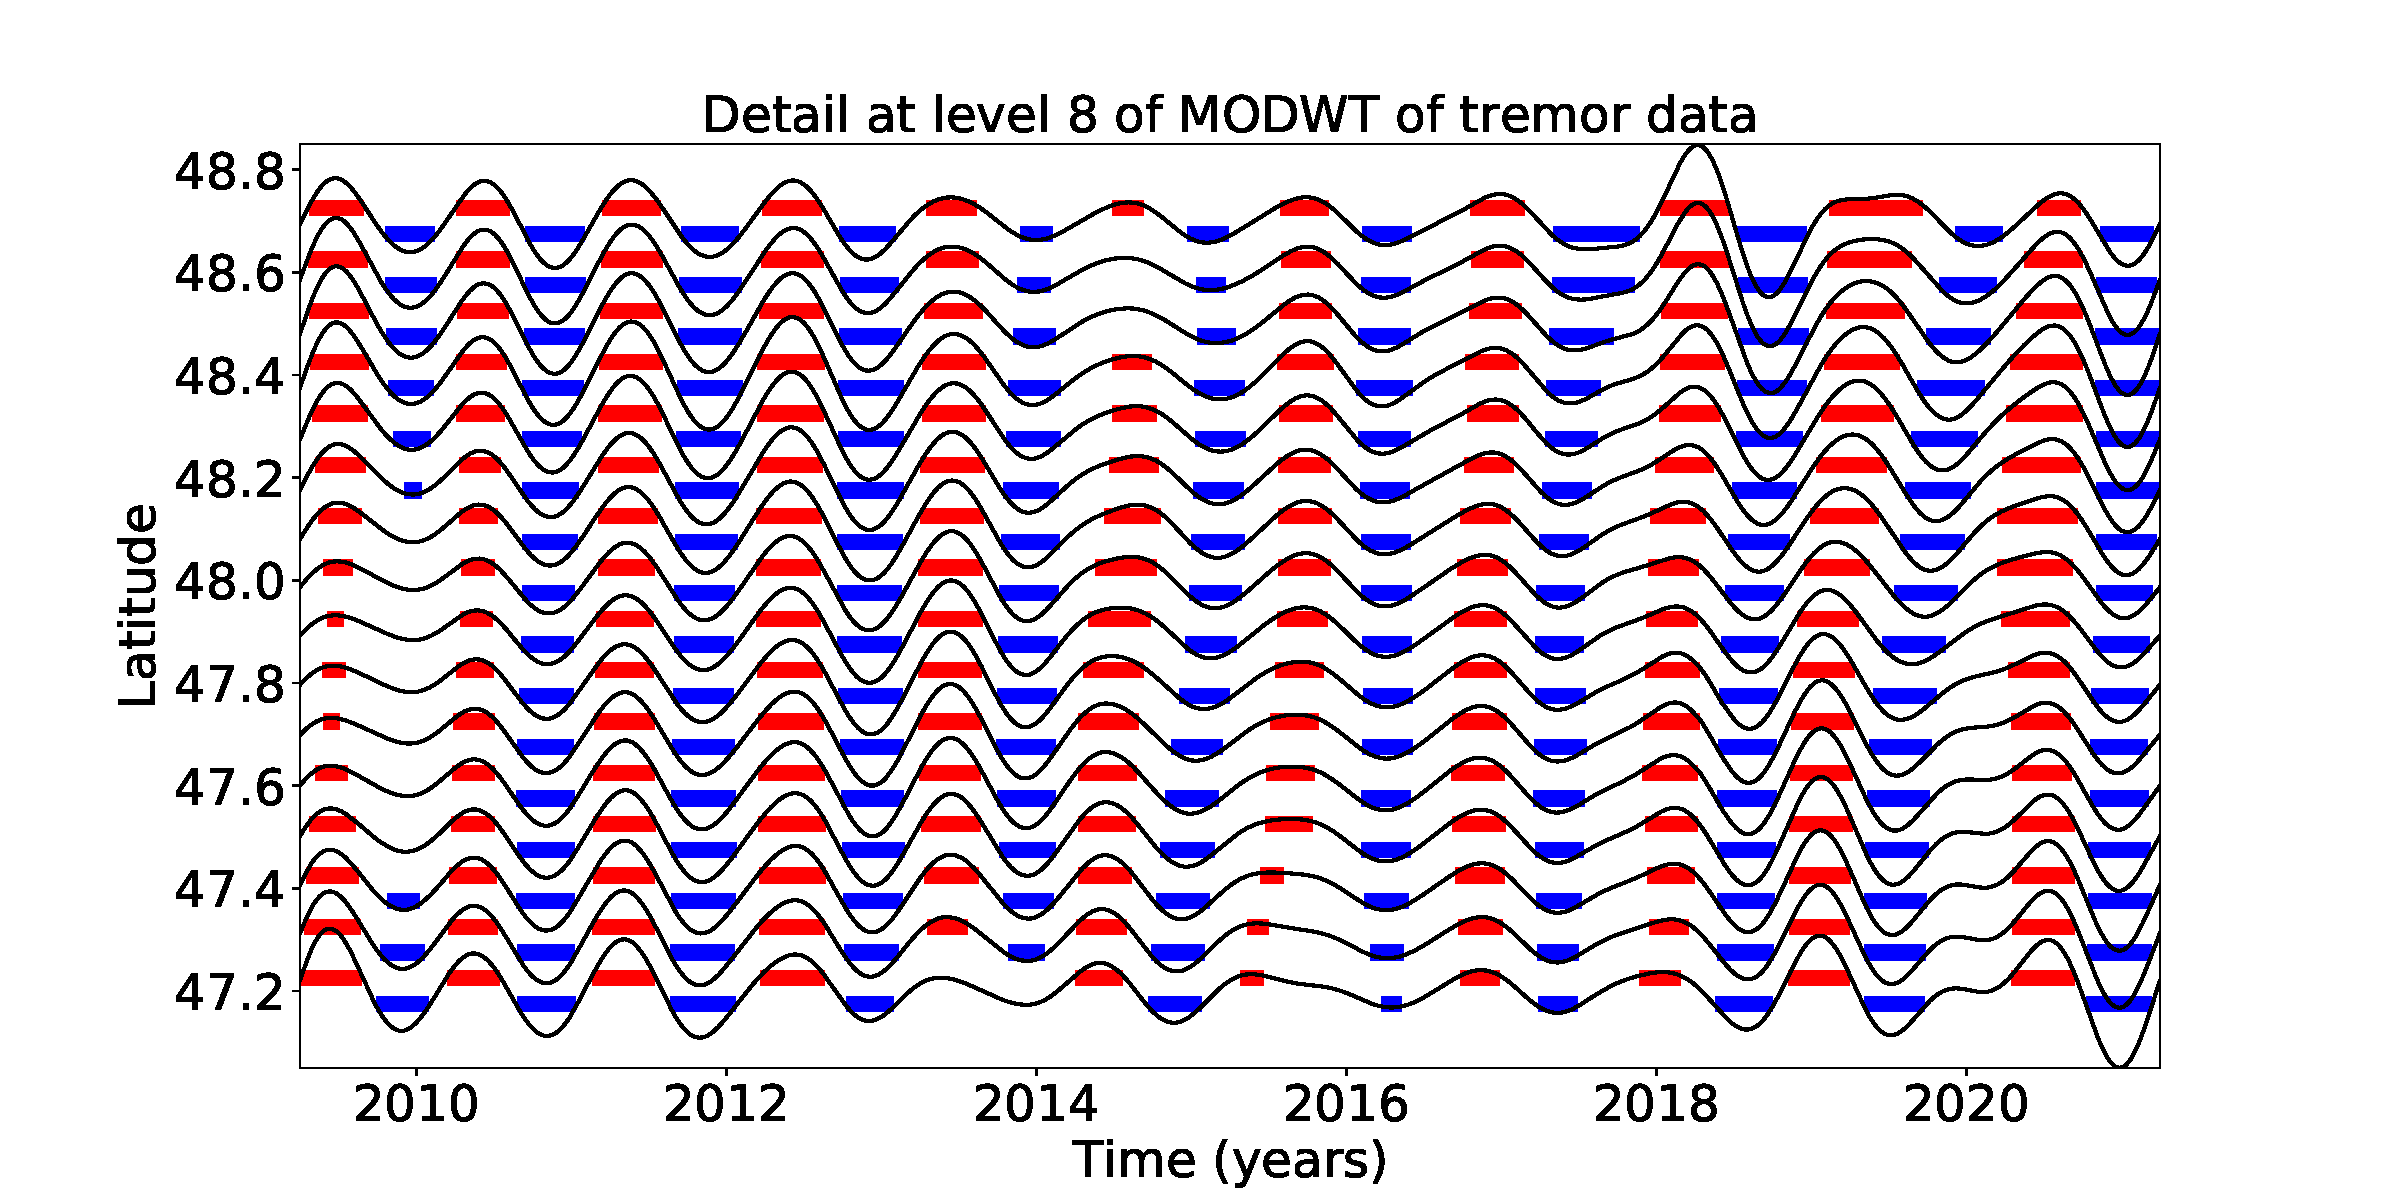
\includegraphics[width=\textwidth, trim={0cm 0cm 0cm 0cm},clip]{figures/tremor_detail_8.pdf}
\caption{Top: Stacked 8th level details of the wavelet decomposition of the displacement over all the GPS stations located in a 50 km radius of a given point, for the 16 locations indicated in Figure 3. Bottom: Opposite of the 8th level detail of the cumulative tremor count in a 50 km radius of a given point for the same 16 locations.}
\label{pngfiguresample}
\end{figure}

Figures 7 and 8 show the same comparison between the wavelet decomposition of the GPS data and the wavelet decomposition of the tremor count data for the 7th level and the 6th level respectively. For the 7th level, we see the same events as for the 8th level, both for the GPS data and the tremor count data. The wavelet decomposition is more noisy for the GPS data in the earliest part of the time series, between 2010 and 2013, but it does not seem that there are more slow slip events visible in the 7th level. \\

\begin{figure}
\noindent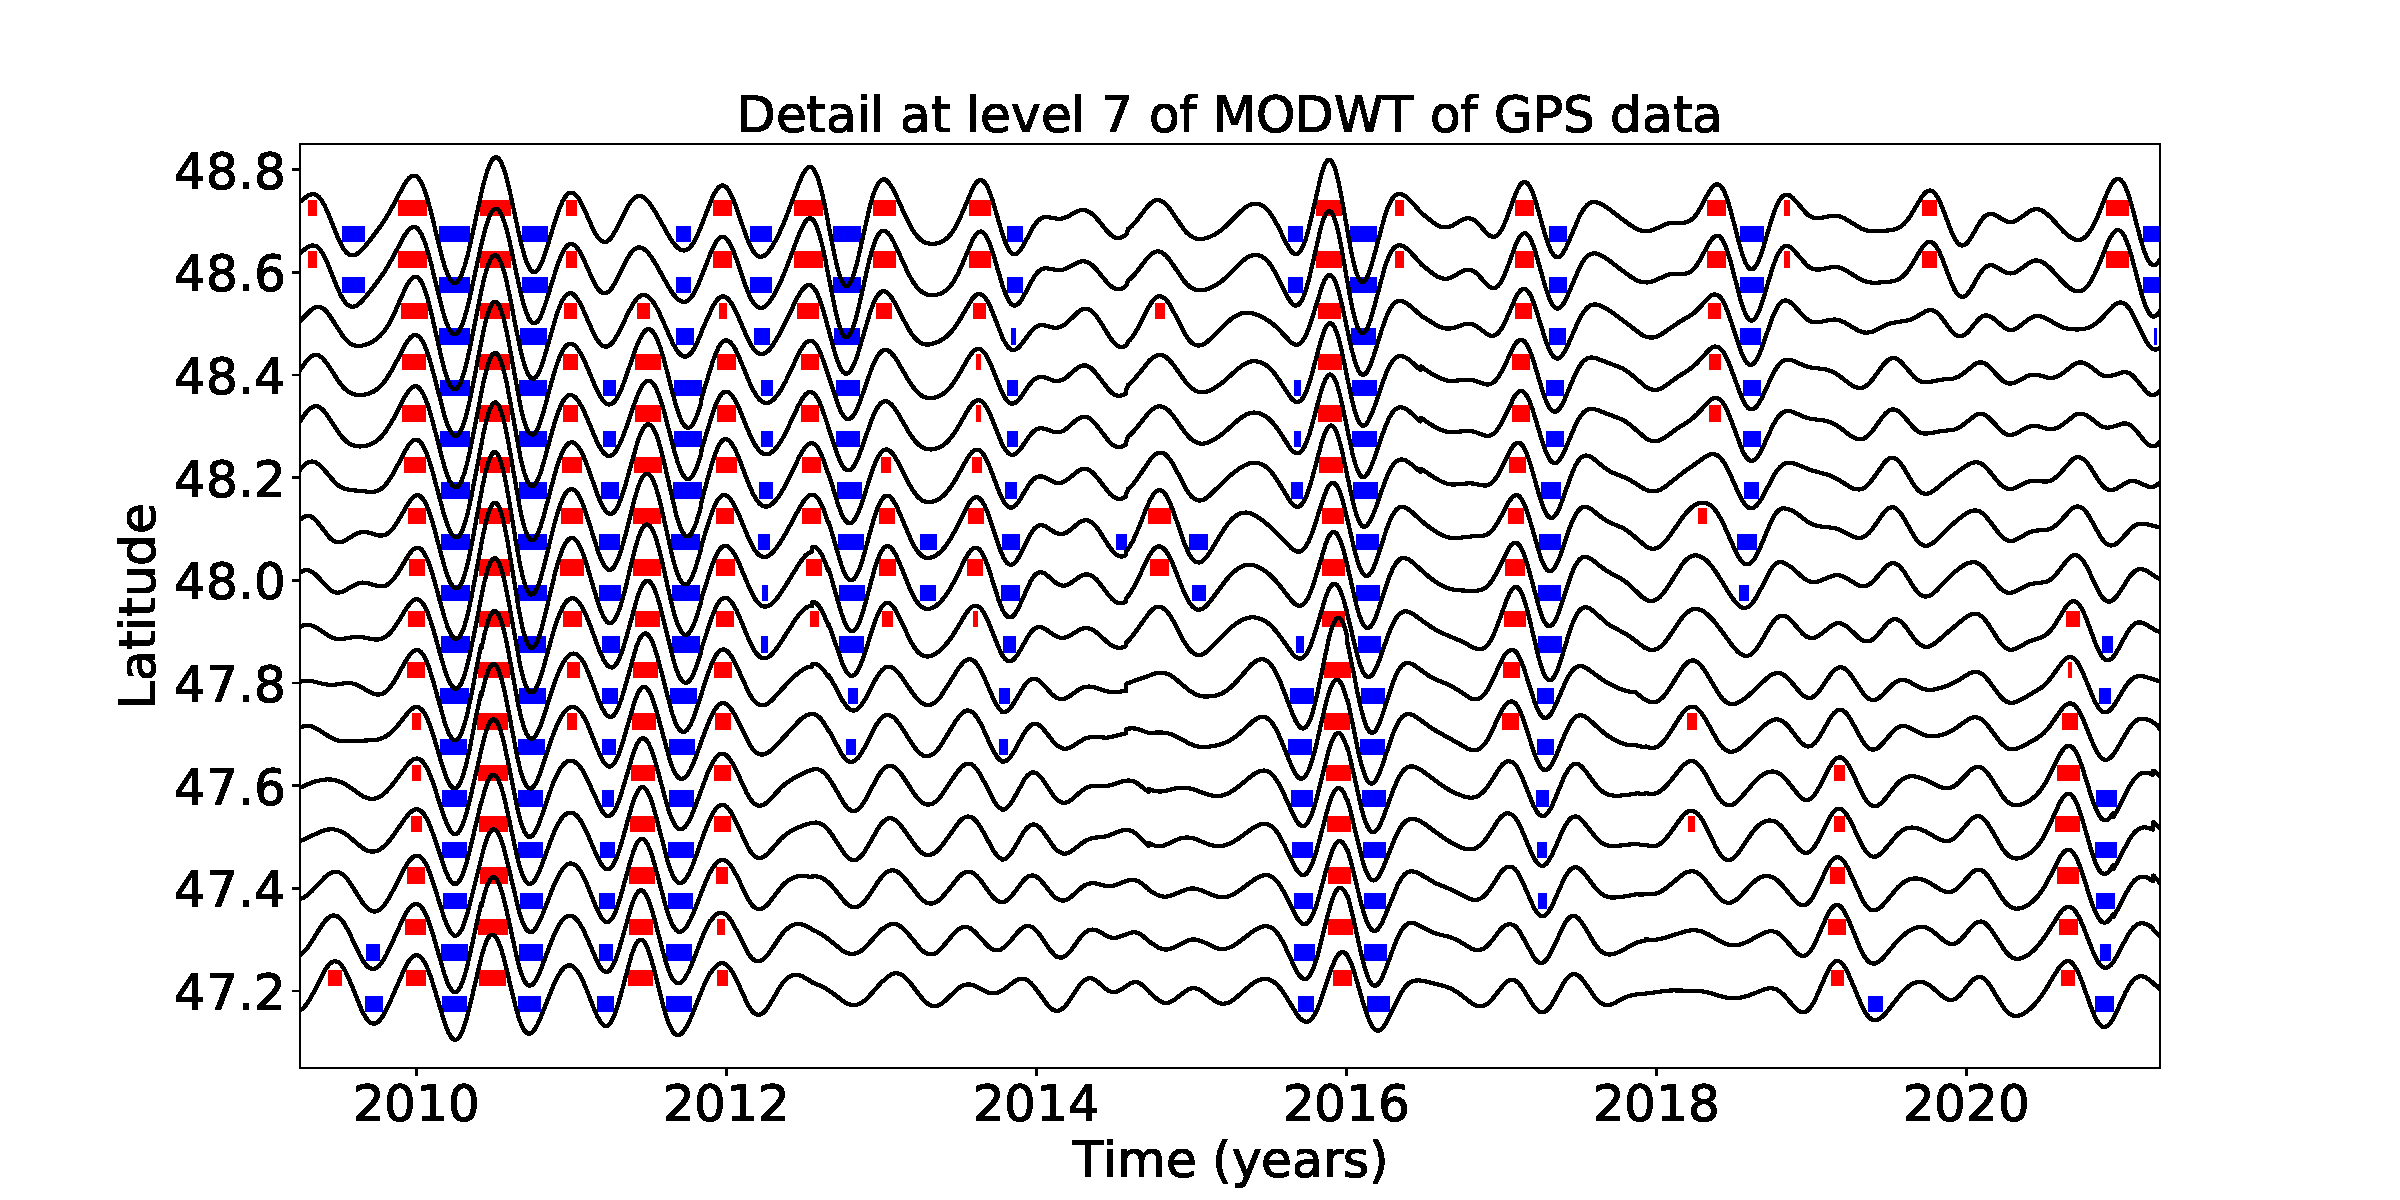
\includegraphics[width=\textwidth, trim={0cm 0cm 0cm 0cm},clip]{figures/GPS_detail_7.pdf}

\noindent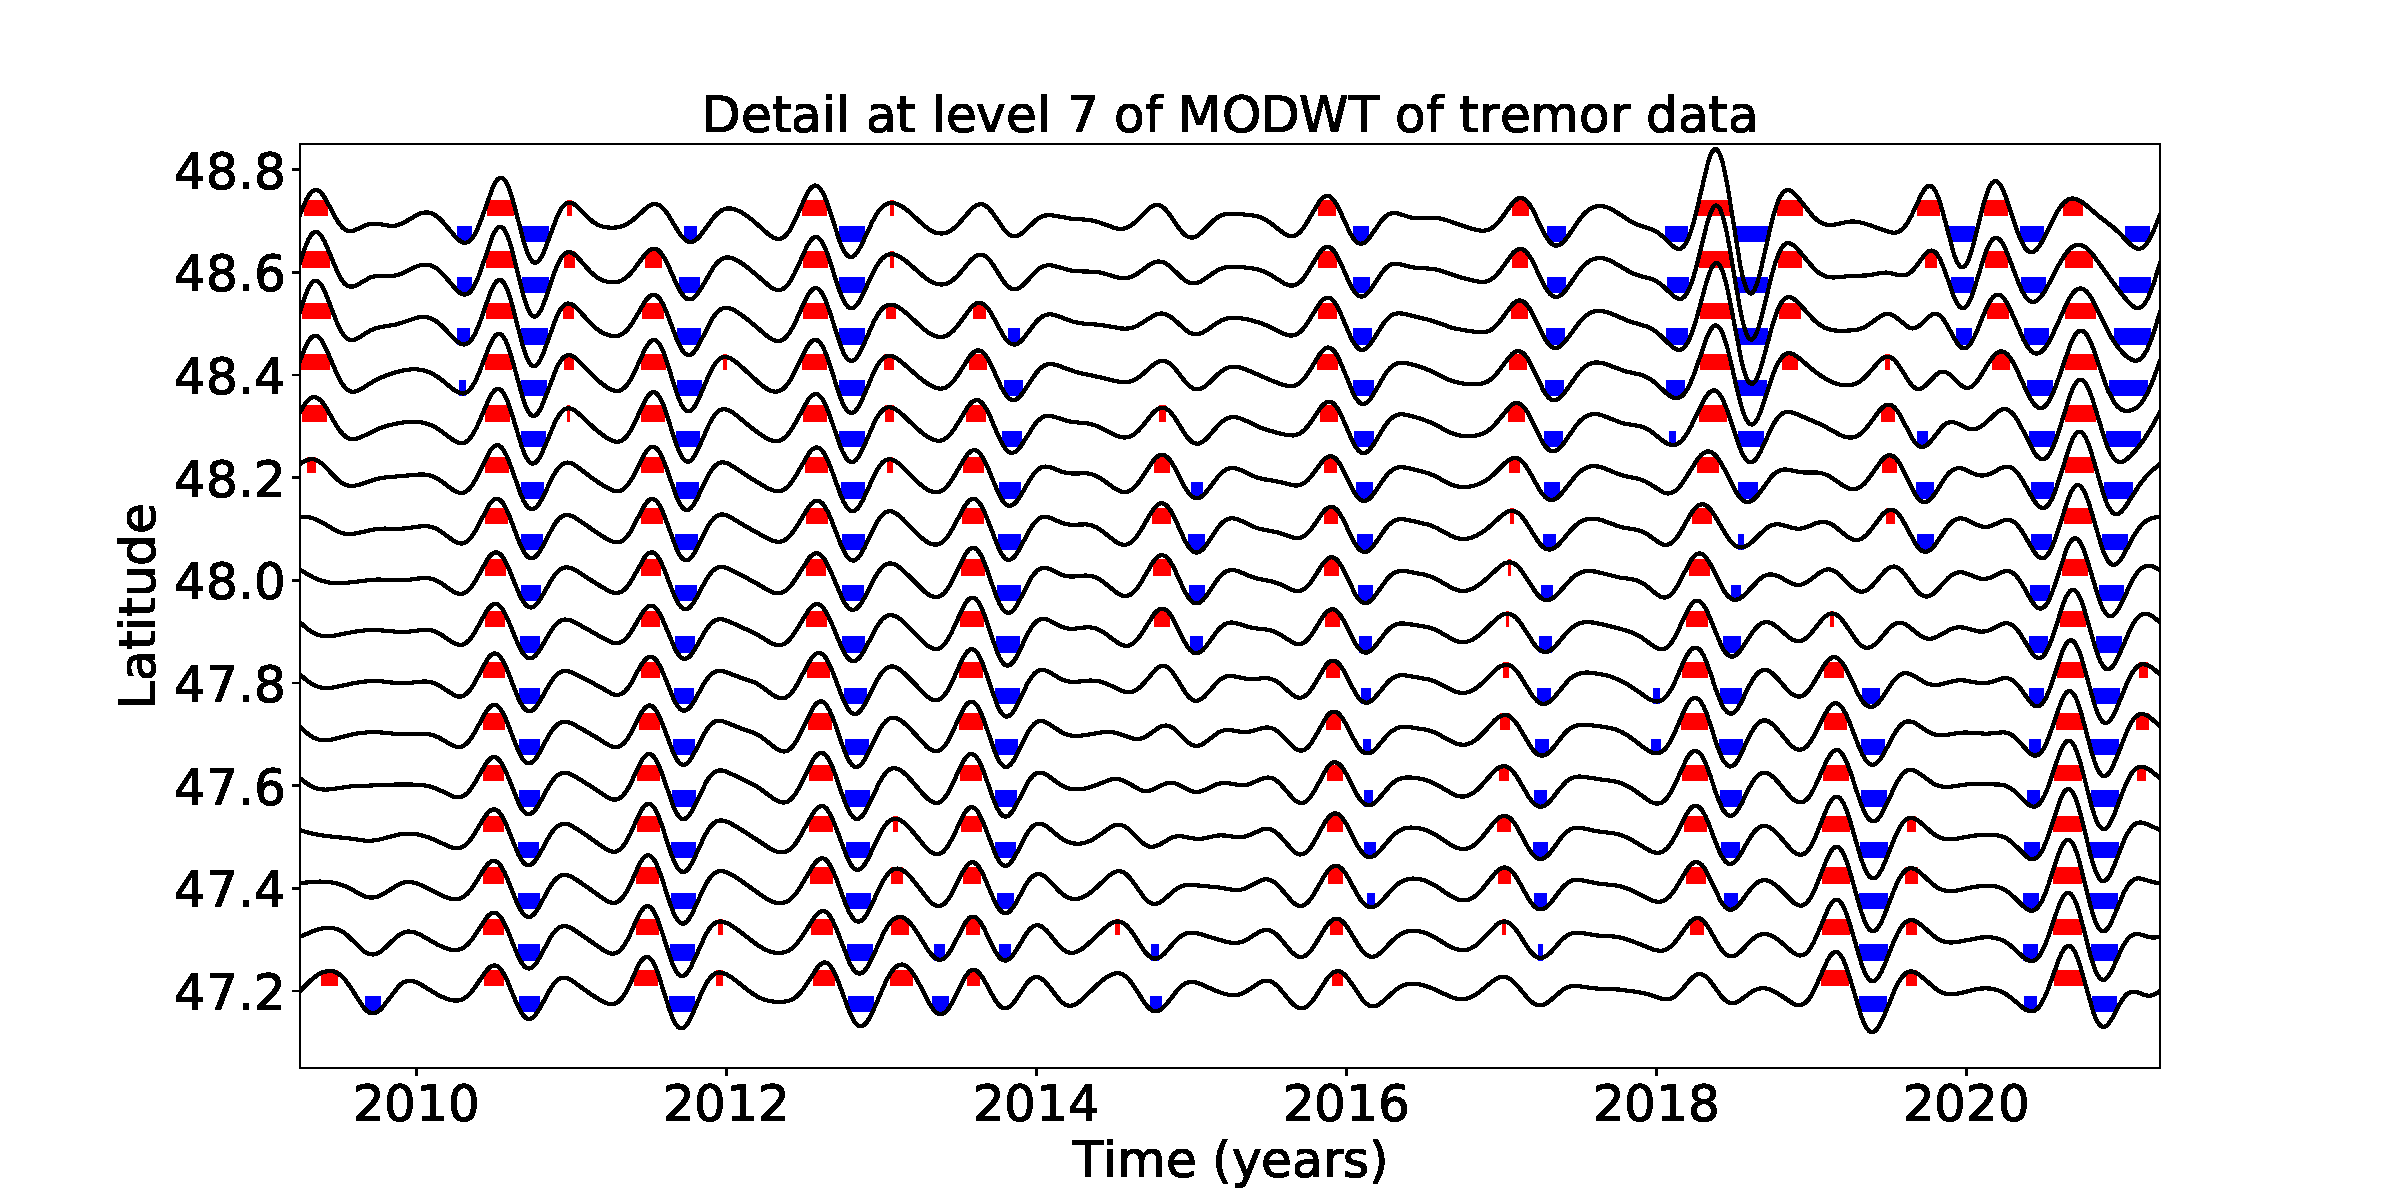
\includegraphics[width=\textwidth, trim={0cm 0cm 0cm 0cm},clip]{figures/tremor_detail_7.pdf}
\caption{Top: Stacked 7th level details of the wavelet decomposition of the displacement over all the GPS stations located in a 50 km radius of a given point, for the 16 locations indicated in Figure 3. Bottom: Opposite of the 7th level detail of the cumulative tremor count in a 50 km radius of a given point for the same 16 locations.}
\label{pngfiguresample}
\end{figure}

For the 6th level detail, we see an additional event in Fall 2009 that is present both in the GPS and the tremor data. There are three small signals in the GPS data in Spring 2012, Fall 2017, and Winter 2020 that are not present in the tremor data, and are probably false detections. To summarize, all the 11 events present on the 7th and 8th level details of the wavelet decomposition are true detections, 12 of the 15 events present on the 6th level detail of the wavelet decomposition are true detections. \\

\begin{figure}
\noindent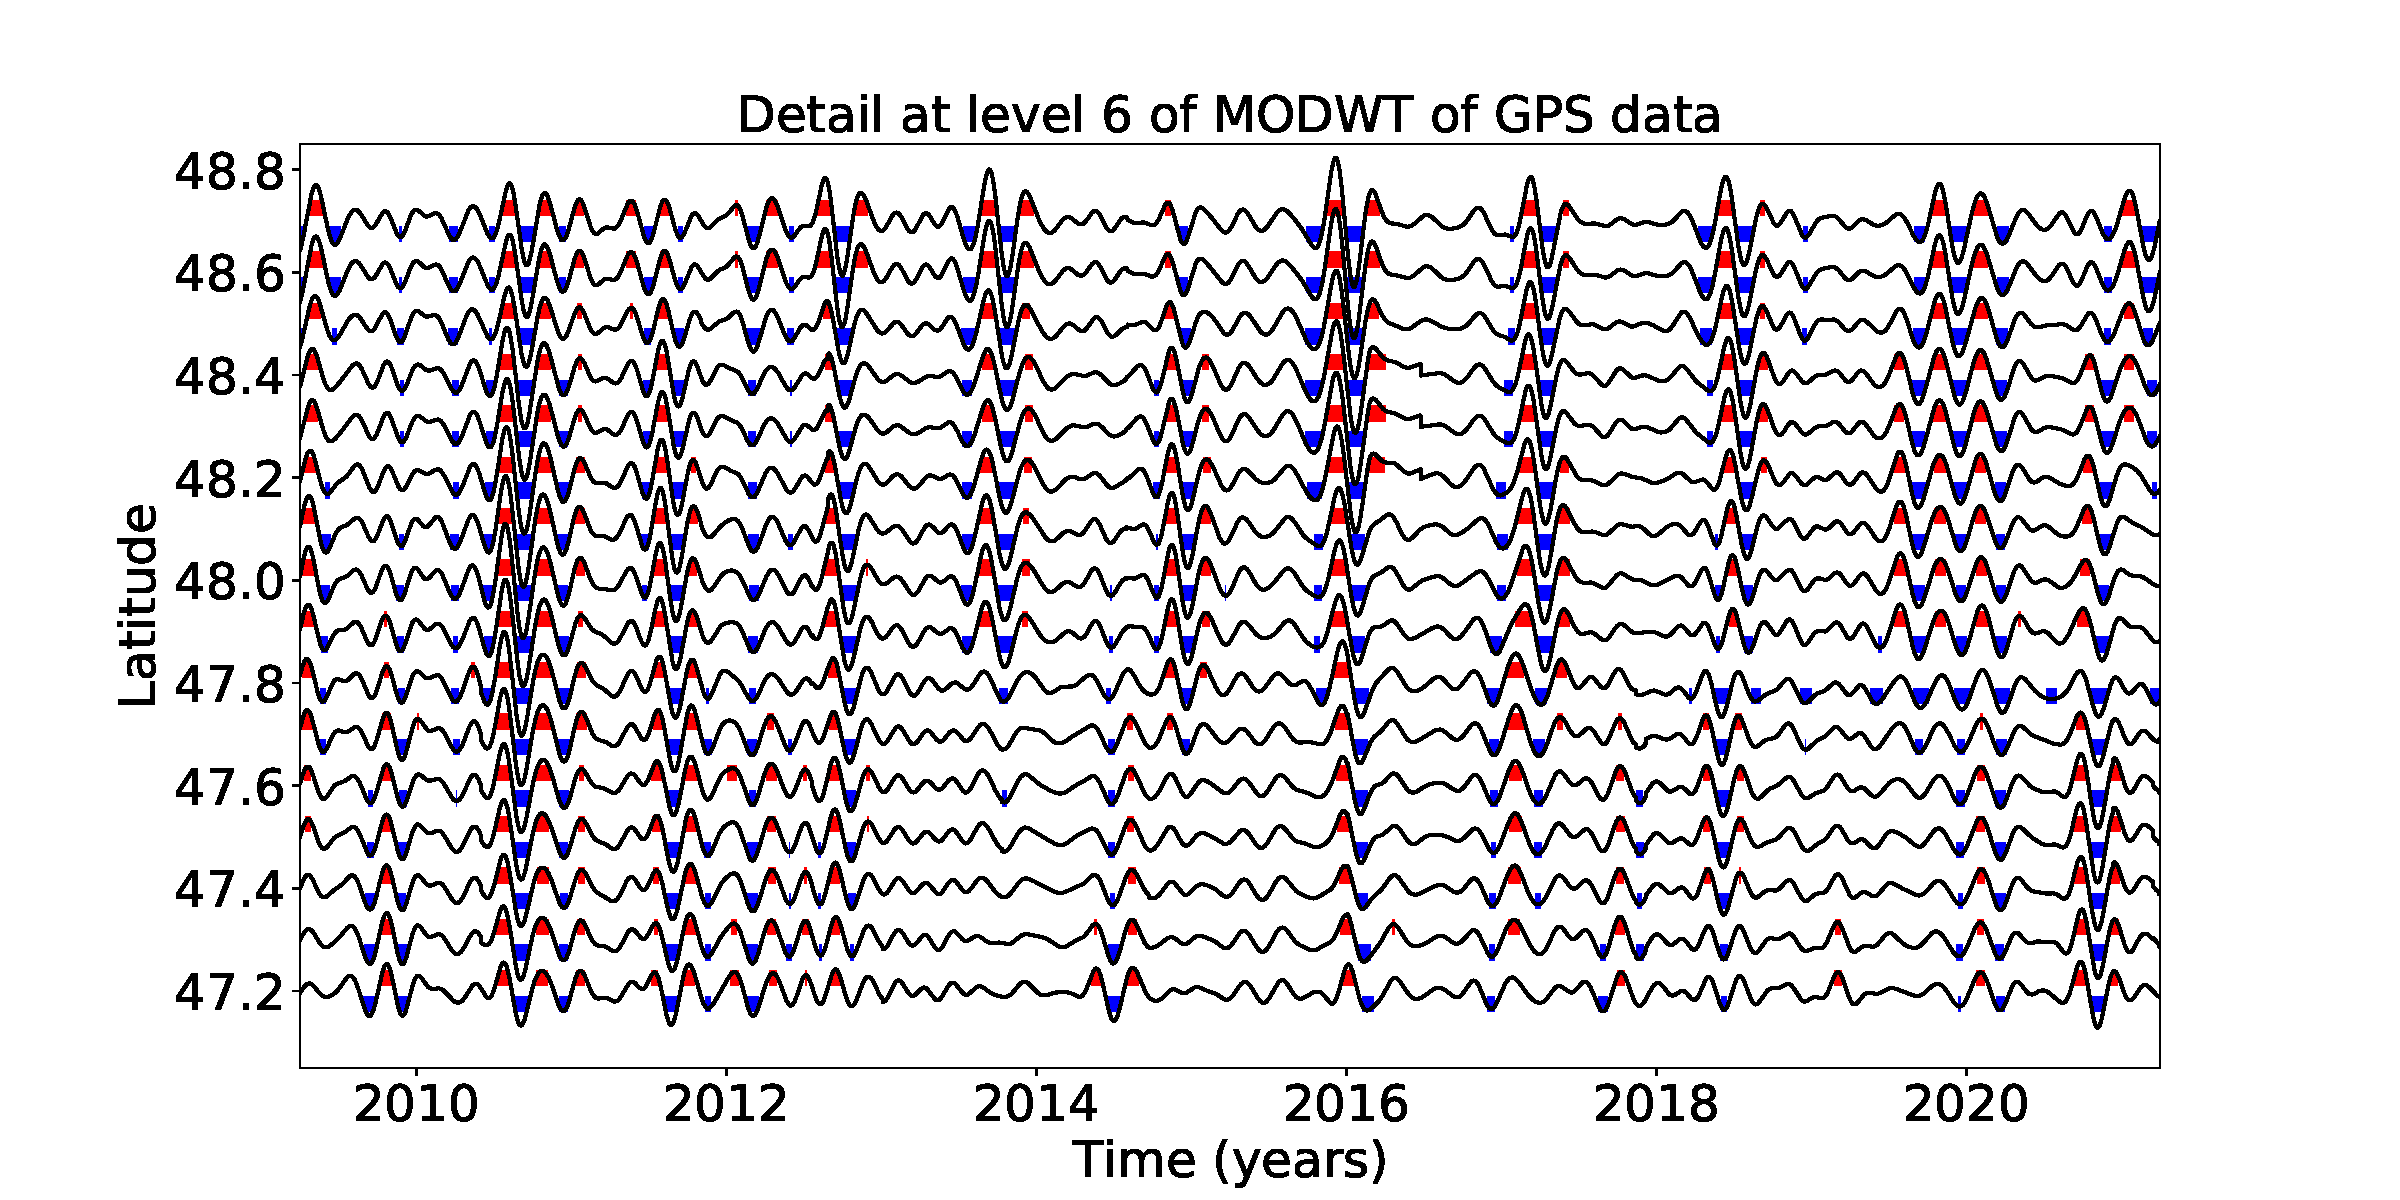
\includegraphics[width=\textwidth, trim={0cm 0cm 0cm 0cm},clip]{figures/GPS_detail_6.pdf}

\noindent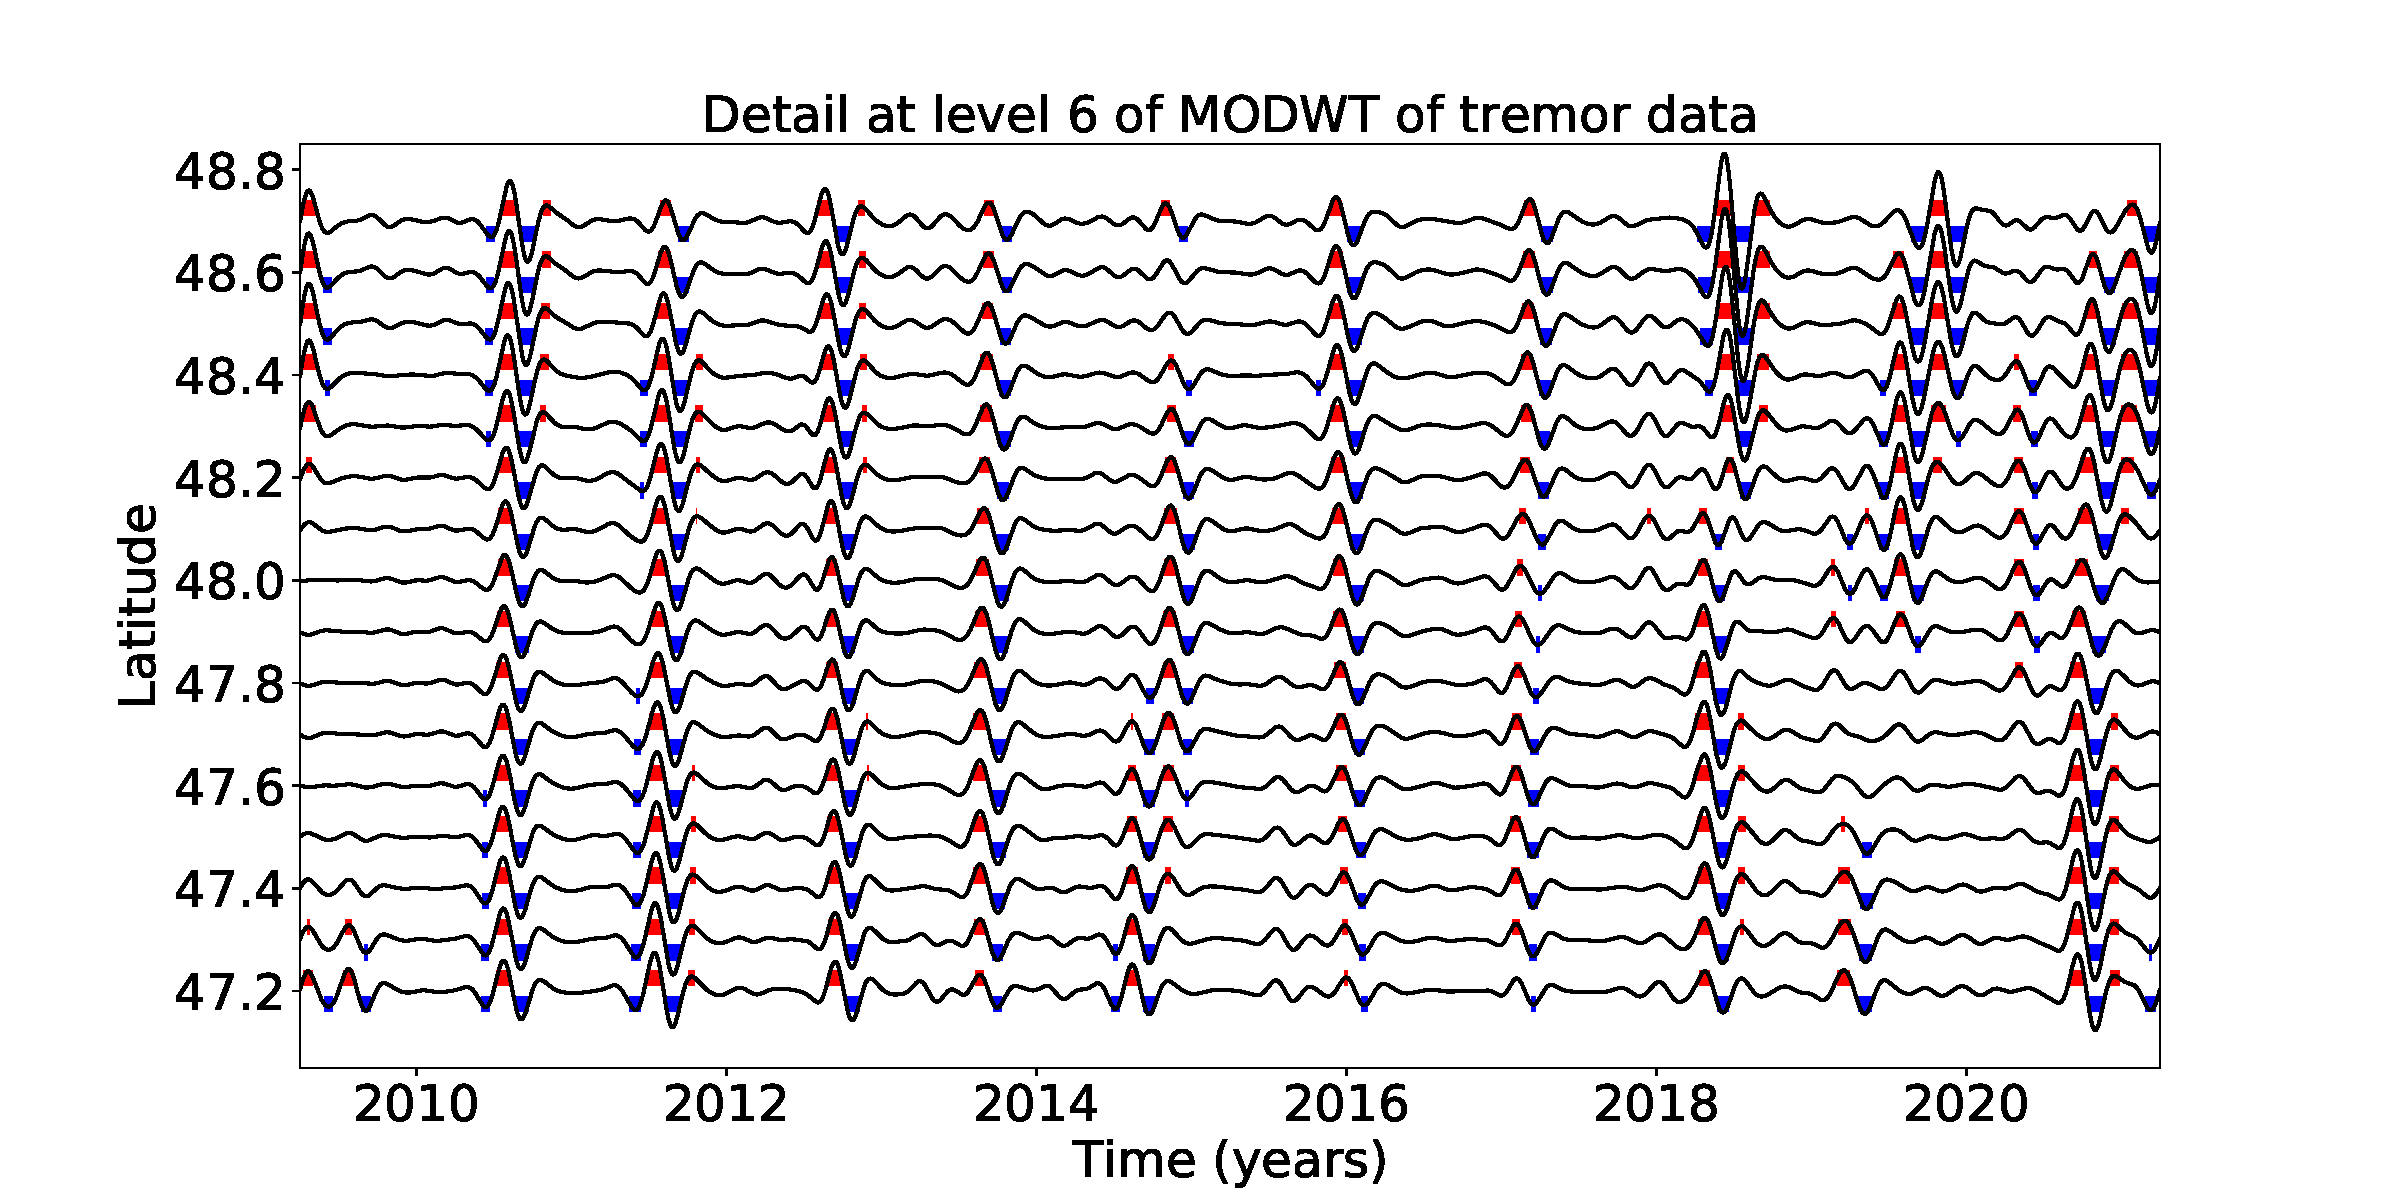
\includegraphics[width=\textwidth, trim={0cm 0cm 0cm 0cm},clip]{figures/tremor_detail_6.pdf}
\caption{Top: Stacked 6th level details of the wavelet decomposition of the displacement over all the GPS stations located in a 50 km radius of a given point, for the 16 locations indicated in Figure 3. Bottom: Opposite of the 6th level detail of the cumulative tremor count in a 50 km radius of a given point for the same 16 locations.}
\label{pngfiguresample}
\end{figure}

\section{Discussion}

In addition to the magnitude 6 events discussed above,  ~\citet{MIC_2019} have also identified several magnitude 5 events using a variational Bayesian Independent Component Analysis (vbICA) decomposition of the signal. As we expect smaller magnitude events to be more visible at smaller time scales of the wavelet decomposition (levels 4 and 5), we verify for all these events whether a signal can be seen at the same time as the time given in their catalog. Most of these magnitude 5 events are also sub-events of bigger magnitude 6 events. Table 1 summarizes for each event its number as indicated in the catalog from ~\citet{MIC_2019}, the beginning and end times as indicated in the catalog from ~\citet{MIC_2019}, whether it is visible at the level 4 of the wavelet decomposition, whether it is visible at the level 5 of the wavelet decomposition, and whether it is part of a bigger magnitude 6 event. All 10 events that are sub-event of a bigger event are visible at both levels 4 and 5. However, this may be due because the bigger event is in at levels 6 to 8, and also at smaller time scales. For the 3 small events that are not part of a bigger event, only one is visible at both time scales, the other two are visible either for level either for level 5 of the wavelet decomposition. Therefore, it is difficult to conclude whether the method can indeed detect events of magnitude 5.

 \begin{table}
 \caption{Magnitude 5 events from ~\citet{MIC_2019}.}
 \centering
 \begin{tabular}{c c c c c}
 \hline
 Event number & Time & Visible at level 4 & Visible at level 5 & Sub-event of bigger event \\
 \hline
 25 & 2010.62-2010.67 & Yes & Yes & Yes \\
 29 & 2011.42-2011.45 & No & Yes & No \\
 31 & 2011.62-2011.68 & Yes & Yes & Yes \\
 32 & 2011.65-2011.68 & Yes & Yes & Yes \\
 35 & 2012.66-2012.72 & Yes & Yes & Yes \\
 42 & 2013.70-2013.78 & Yes & Yes & Yes \\
 44 & 2014.12-2014-20 & Yes & No & No \\
 45 & 2014.40-2014.48 & Yes & Yes & No \\
 49 & 2014.66-2014.71 & Yes & Yes & Yes \\
 52 & 2014.91-2014.95 & Yes & Yes & Yes \\
 57 & 2015.98-2016.08 & Yes & Yes & Yes \\
 60 & 2017.11-2017.15 & Yes & Yes & Yes \\
 61 & 2017.20-2017.24 & Yes & Yes & Yes \\
 \hline
 \end{tabular}
 \end{table}


\section{Conclusion}

%%

%  Numbered lines in equations:
%  To add line numbers to lines in equations,
%  \begin{linenomath*}
%  \begin{equation}
%  \end{equation}
%  \end{linenomath*}



%% Enter Figures and Tables near as possible to where they are first mentioned:
%
% DO NOT USE \psfrag or \subfigure commands.
%
% Figure captions go below the figure.
% Table titles go above tables;  other caption information
%  should be placed in last line of the table, using
% \multicolumn2l{$^a$ This is a table note.}
%
%----------------
% EXAMPLE FIGURE
%
% \begin{figure}[h]
% \centering
% when using pdflatex, use pdf file:
% \includegraphics[natwidth=800px,natheight=600px]{figsamp.pdf}
%
% when using dvips, use .eps file:
% \includegraphics[natwidth=800px,natheight=600px]{figsamp.eps}
%
% \caption{Short caption}
% \label{figone}
%  \end{figure}
%
% We recommend that you provide the native width and height (natwidth, natheight) of your figures.
% Specifying native dimensions ensures that your figures are properly scaled
%
%
% ---------------
% EXAMPLE TABLE
%
% \begin{table}
% \caption{Time of the Transition Between Phase 1 and Phase 2$^{a}$}
% \centering
% \begin{tabular}{l c}
% \hline
%  Run  & Time (min)  \\
% \hline
%   $l1$  & 260   \\
%   $l2$  & 300   \\
%   $l3$  & 340   \\
%   $h1$  & 270   \\
%   $h2$  & 250   \\
%   $h3$  & 380   \\
%   $r1$  & 370   \\
%   $r2$  & 390   \\
% \hline
% \multicolumn{2}{l}{$^{a}$Footnote text here.}
% \end{tabular}
% \end{table}

%% SIDEWAYS FIGURE and TABLE
% AGU prefers the use of {sidewaystable} over {landscapetable} as it causes fewer problems.
%
% \begin{sidewaysfigure}
% \includegraphics[width=20pc]{figsamp}
% \caption{caption here}
% \label{newfig}
% \end{sidewaysfigure}
%
%  \begin{sidewaystable}
%  \caption{Caption here}
% \label{tab:signif_gap_clos}
%  \begin{tabular}{ccc}
% one&two&three\\
% four&five&six
%  \end{tabular}
%  \end{sidewaystable}

%% If using numbered lines, please surround equations with \begin{linenomath*}...\end{linenomath*}
%\begin{linenomath*}
%\begin{equation}
%y|{f} \sim g(m, \sigma),
%\end{equation}
%\end{linenomath*}

%%% End of body of article

%%%%%%%%%%%%%%%%%%%%%%%%%%%%%%%%
%% Optional Appendix goes here
%
% The \appendix command resets counters and redefines section heads
%
% After typing \appendix
%
%\section{Here Is Appendix Title}
% will show
% A: Here Is Appendix Title
%
%\appendix
%\section{Here is a sample appendix}

%%%%%%%%%%%%%%%%%%%%%%%%%%%%%%%%%%%%%%%%%%%%%%%%%%%%%%%%%%%%%%%%
%
% Optional Glossary, Notation or Acronym section goes here:
%
%%%%%%%%%%%%%%
% Glossary is only allowed in Reviews of Geophysics
%  \begin{glossary}
%  \term{Term}
%   Term Definition here
%  \term{Term}
%   Term Definition here
%  \term{Term}
%   Term Definition here
%  \end{glossary}

%
%%%%%%%%%%%%%%
% Acronyms
%   \begin{acronyms}
%   \acro{Acronym}
%   Definition here
%   \acro{EMOS}
%   Ensemble model output statistics
%   \acro{ECMWF}
%   Centre for Medium-Range Weather Forecasts
%   \end{acronyms}

%
%%%%%%%%%%%%%%
% Notation
%   \begin{notation}
%   \notation{$a+b$} Notation Definition here
%   \notation{$e=mc^2$}
%   Equation in German-born physicist Albert Einstein's theory of special
%  relativity that showed that the increased relativistic mass ($m$) of a
%  body comes from the energy of motion of the body—that is, its kinetic
%  energy ($E$)—divided by the speed of light squared ($c^2$).
%   \end{notation}




%%%%%%%%%%%%%%%%%%%%%%%%%%%%%%%%%%%%%%%%%%%%%%%%%%%%%%%%%%%%%%%%
%
%  ACKNOWLEDGMENTS
%
% The acknowledgments must list:
%
% >>>>	A statement that indicates to the reader where the data
% 	supporting the conclusions can be obtained (for example, in the
% 	references, tables, supporting information, and other databases).
%
% 	All funding sources related to this work from all authors
%
% 	Any real or perceived financial conflicts of interests for any
%	author
%
% 	Other affiliations for any author that may be perceived as
% 	having a conflict of interest with respect to the results of this
% 	paper.
%
%
% It is also the appropriate place to thank colleagues and other contributors.
% AGU does not normally allow dedications.


\acknowledgments
Enter acknowledgments, including your data availability statement, here.


%% ------------------------------------------------------------------------ %%
%% References and Citations

%%%%%%%%%%%%%%%%%%%%%%%%%%%%%%%%%%%%%%%%%%%%%%%
% BibTeX is preferred:
%
\bibliography{bibliography.bib}
%
% don't specify bibliographystyle
%%%%%%%%%%%%%%%%%%%%%%%%%%%%%%%%%%%%%%%%%%%%%%%



% Please use ONLY \citet and \citep for reference citations.
% DO NOT use other cite commands (e.g., \cite, \citeyear, \nocite, \citealp, etc.).
%% Example \citet and \citep:
%  ...as shown by \citet{Boug10}, \citet{Buiz07}, \citet{Fra10},
%  \citet{Ghel00}, and \citet{Leit74}.

%  ...as shown by \citep{Boug10}, \citep{Buiz07}, \citep{Fra10},
%  \citep{Ghel00, Leit74}.

%  ...has been shown \citep [e.g.,][]{Boug10,Buiz07,Fra10}.


\end{document}



More Information and Advice:

%% ------------------------------------------------------------------------ %%
%
%  SECTION HEADS
%
%% ------------------------------------------------------------------------ %%

% Capitalize the first letter of each word (except for
% prepositions, conjunctions, and articles that are
% three or fewer letters).

% AGU follows standard outline style; therefore, there cannot be a section 1 without
% a section 2, or a section 2.3.1 without a section 2.3.2.
% Please make sure your section numbers are balanced.
% ---------------
% Level 1 head
%
% Use the \section{} command to identify level 1 heads;
% type the appropriate head wording between the curly
% brackets, as shown below.
%
%An example:
%\section{Level 1 Head: Introduction}
%
% ---------------
% Level 2 head
%
% Use the \subsection{} command to identify level 2 heads.
%An example:
%\subsection{Level 2 Head}
%
% ---------------
% Level 3 head
%
% Use the \subsubsection{} command to identify level 3 heads
%An example:
%\subsubsection{Level 3 Head}
%
%---------------
% Level 4 head
%
% Use the \subsubsubsection{} command to identify level 3 heads
% An example:
%\subsubsubsection{Level 4 Head} An example.
%
%% ------------------------------------------------------------------------ %%
%
%  IN-TEXT LISTS
%
%% ------------------------------------------------------------------------ %%
%
% Do not use bulleted lists; enumerated lists are okay.
% \begin{enumerate}
% \item
% \item
% \item
% \end{enumerate}
%
%% ------------------------------------------------------------------------ %%
%
%  EQUATIONS
%
%% ------------------------------------------------------------------------ %%

% Single-line equations are centered.
% Equation arrays will appear left-aligned.

Math coded inside display math mode \[ ...\]
 will not be numbered, e.g.,:
 \[ x^2=y^2 + z^2\]

 Math coded inside \begin{equation} and \end{equation} will
 be automatically numbered, e.g.,:
 \begin{equation}
 x^2=y^2 + z^2
 \end{equation}


% To create multiline equations, use the
% \begin{eqnarray} and \end{eqnarray} environment
% as demonstrated below.
\begin{eqnarray}
  x_{1} & = & (x - x_{0}) \cos \Theta \nonumber \\
        && + (y - y_{0}) \sin \Theta  \nonumber \\
  y_{1} & = & -(x - x_{0}) \sin \Theta \nonumber \\
        && + (y - y_{0}) \cos \Theta.
\end{eqnarray}

%If you don't want an equation number, use the star form:
%\begin{eqnarray*}...\end{eqnarray*}

% Break each line at a sign of operation
% (+, -, etc.) if possible, with the sign of operation
% on the new line.

% Indent second and subsequent lines to align with
% the first character following the equal sign on the
% first line.

% Use an \hspace{} command to insert horizontal space
% into your equation if necessary. Place an appropriate
% unit of measure between the curly braces, e.g.
% \hspace{1in}; you may have to experiment to achieve
% the correct amount of space.


%% ------------------------------------------------------------------------ %%
%
%  EQUATION NUMBERING: COUNTER
%
%% ------------------------------------------------------------------------ %%

% You may change equation numbering by resetting
% the equation counter or by explicitly numbering
% an equation.

% To explicitly number an equation, type \eqnum{}
% (with the desired number between the brackets)
% after the \begin{equation} or \begin{eqnarray}
% command.  The \eqnum{} command will affect only
% the equation it appears with; LaTeX will number
% any equations appearing later in the manuscript
% according to the equation counter.
%

% If you have a multiline equation that needs only
% one equation number, use a \nonumber command in
% front of the double backslashes (\\) as shown in
% the multiline equation above.

% If you are using line numbers, remember to surround
% equations with \begin{linenomath*}...\end{linenomath*}

%  To add line numbers to lines in equations:
%  \begin{linenomath*}
%  \begin{equation}
%  \end{equation}
%  \end{linenomath*}



